\newpage
\section{Geometric Priors}
\label{sec:geom_priors}
Modern data analysis is synonymous with high-dimensional learning.  
While the simple arguments of Section~\ref{sec:inductive} reveal the impossibility of learning 
from generic high-dimensional data as a result of the curse of dimensionality, 
there is hope for physically-structured data, where we can employ two fundamental principles: {\em symmetry} and {\em scale separation}. 
In the settings considered in this text, this additional structure will usually come from the structure of the domain underlying the input signals: 
we will assume that our machine learning system operates on \emph{signals} (functions) on some domain $\Omega$. 
%
While in many cases linear combinations of points on $\Omega$ is not well-defined\marginnote{$\Omega$ must be a vector space in order for an expression $\alpha u + \beta v$ to make sense.}, we can linearly combine signals on it, i.e., the space of signals forms a vector space. 
Moreover, since we can define an inner product between signals, this space is a {\em Hilbert space}.

\begin{tcolorbox}[width=\linewidth,
                  boxsep=0pt,
                  left=7.5pt,
                  right=7.5pt,
                  top=7.5pt,
                  bottom=7.5pt,
                  arc=0pt,
                  boxrule=0pt,toprule=0pt,
                  colback=boxgray,
                  ]%%

The space of $\mathcal{C}$-valued signals on $\Omega$ 
\marginnote{When $\Omega$ has some additional structure, we may further restrict the kinds of signals in $\mathcal{X}(\Omega, \mathcal{C})$. For example, when $\Omega$ is a smooth manifold, we may require the signals to be smooth. 
Whenever possible, we will omit the range $\mathcal{C}$ for brevity. 
} %can impose smoothness on the signals.}% For instance, when $\Omega$ is a smooth manifold we may require signals in $\mathcal{X}(\Omega, \mathcal{C})$ to be smooth.}
(for $\Omega$ a set, possibly with additional structure, and $\mathcal{C}$ a vector space, whose dimensions are called \emph{channels}) 
\begin{equation}
    \mathcal{X}(\Omega, \mathcal{C}) = \{ x : \Omega \rightarrow \mathcal{C} \}
\end{equation}
%
is a function space that has a vector space structure. 
%In particular, it satisfies the distributivity property 
Addition and scalar multiplication of signals is defined as:
\begin{equation*}
    (\alpha x + \beta y)(u) = \alpha x(u) + \beta y(u) \quad \text{for all} \quad u\in \Omega,
\end{equation*}
with real scalars $\alpha, \beta$. % are vectors, and $u \in \Omega$.
%
Given an inner product $\langle v, w \rangle_\mathcal{C}$ on $\mathcal{C}$ and a measure\marginnote{When the domain $\Omega$ is discrete, $\mu$ can be chosen as the {\em counting measure}, in which case the integral becomes a sum. In the following, we will omit the measure and use $\mathrm{d}u$ for brevity.  } $\mu$ on $\Omega$ (with respect to which we can define an integral), we can define an inner product on $\mathcal{X}(\Omega, \mathcal{C})$ as 
\begin{equation}
    \langle x, y \rangle = \int_{\Omega} \langle x(u), \, y(u) \rangle_{\mathcal{C}} \; \mathrm{d}\mu(u).
    \label{eqn:innerprod}
\end{equation}
\end{tcolorbox}

%we will assume that $f$ operates on $\mathcal{C}$-valued signals $\mathcal{X}(\Omega, \mathcal{C}) = \{x: \Omega \rightarrow \mathcal{C} \}$, where $\Omega$ is some input domain and $\mathcal{C}$ is a vector space, typically $\mathcal{C} = \R^s$ for a signal with $s$ channels.
%\marginnote{For the sake of simplicity, we will often assume scalar-valued signals, i.e., $s=1$. }
%We note that $\mathcal{X}(\Omega, \mathcal{C})$ is a vector space, with addition and scalar multiplication defined pointwise (i.e. $(f + f')(x) = f(x) + f(x')$ and $(\alpha f)(x) = \alpha f(x)$).

As a typical illustration, take $\Omega = \mathbb{Z}_n\times \mathbb{Z}_n$ to be a two-dimensional $n\times n$ grid, $x$ an RGB image (i.e. a signal $x : \Omega \rightarrow \R^3$), and $f$ a function (such as a single-layer Perceptron) operating on $3n^2$-dimensional inputs. 
%
As we will see in the following with greater detail, the domain $\Omega$ is usually endowed with certain geometric structure and symmetries. %symmetric structure (in our example, rotational and translational symmetry) that is manifested both in signals $x$ defined on this domain as well as in functions $f$ acting on such signals. 
%
Scale separation results from our ability to preserve important characteristics of the signal when transferring it onto a coarser version of the domain (in our example, subsampling the image by coarsening the underlying grid). 


We will show that both principles, to which we will generically refer as {\em geometric priors}, are prominent in most modern deep learning architectures. In the case of images considered above, geometric priors are built into Convolutional Neural Networks (CNNs) in the form of convolutional filters with shared weights (exploiting translational symmetry) and pooling (exploiting scale separation). 
%
Extending these ideas to other domains such as graphs and manifolds and showing how geometric priors emerge from fundamental principles is the main goal of Geometric Deep Learning and the {\em leitmotif} of our text.   



\subsection{Symmetries, Representations, and Invariance}
\label{sec:symmetries}

%Symmetries are a foundational principle of physics, providing a strong constraint on the form of physical laws.
%In the context of machine learning, symmetries also provide key regularity priors that allow to break the curse of dimensionality and enable efficient high-dimensional learning. 

Informally, a {\em symmetry} of an object or system is a transformation that leaves a certain property of said object or system unchanged or {\em invariant}.
Such transformations may be either smooth, continuous, or discrete.
%A canonical example for continuous symmetries in physics is Lagrangian mechanics, which states that the laws of motion are preserved under rigid transformations of the observer's point of view. 
%
Symmetries are ubiquitous in many machine learning tasks.
For example, in computer vision the object category is unchanged by shifts, so shifts are symmetries in the problem of visual object classification.
%one is often interested in classifying  objects in images independently of their position, a setting referred to as {\em translation invariant}. 
%
%classification through translation invariance, or 
In computational chemistry, the task of predicting properties of molecules independently of their orientation in space requires {\em rotational invariance}. 
%
Discrete symmetries emerge naturally when describing particle systems where particles do not have canonical ordering and thus can be arbitrarily permuted, as well as
%through permutations, 
%or also 
in many dynamical systems, via the time-reversal symmetry (such as systems in detailed balance or the Newton's second law of motion). %\marginnote{ADD COMMENT on Newton's law} % may not be necessary imo
%
As we will see in Section~\ref{sec:proto-graphs}, permutation symmetries are also central to the analysis of graph-structured data. % and will be a prominent topic in this book. 

\paragraph{Symmetry groups}
The set of symmetries of an object satisfies a number of properties. 
%which make this set into an algebraic structure called a \emph{symmetry group}.
%Symmetries lend themselves to a rich and powerful mathematical characterization.
%More specifically, the set of symmetries of a given object forms an algebraic object called a symmetry group.
First, symmetries may be combined to obtain new symmetries: if $\fg$ and $\fh$ are two symmetries,
%transformations of a system that leave it unchanged, 
then their  compositions $\fg \circ \fh$ and $\fh \circ \fg$
%\marginnote{From hereon we will denote composition of group elements by $\fg \fh$, leaving out the $\circ$ symbol.}
\marginnote{We will follow the juxtaposition notation convention used in group theory, $\fg \circ \fh = \fg \fh$, which should be read right-to-left: we first apply $\fh$ and then $\fg$. The order is important, as in many cases symmetries are non-commutative. 
%
Readers familiar with Lie groups might be disturbed by our choice to use the Fraktur font to denote group elements, as it is a  common notation of Lie algebras.
} are also symmetries.
The reason is that if both transformations leave the object invariant, then so does the composition of transformations, and hence the composition is also a symmetry.
%\marginnote{This property is called {\em closure} in group theory.} 
Furthermore, symmetries are always invertible, and the inverse is also a symmetry.
%Together with {\em associativity} $(\fg \circ \fh) \circ \ff = \fg \circ (\fh \circ \ff)$ of the composition operation and existence of unique {\em identity} ($\exists!\fe \in \fG$ such that $\fe \circ \fg = \fg \circ \fe = \fe$ for all $\fg \in \fG$) and {\em inverse} (for any $\fg \in \fG$, $\exists! \fg^{-1} \in \fG$ such that $\fg\circ \fg^{-1} = \fg^{-1}\circ \fg = \fe$), it formally defines a group.} 
This shows that the collection of all symmetries form an algebraic object known as a {\em group}. Since these objects will be a centerpiece of the mathematical model of Geometric Deep Learning, they deserve a formal definition and detailed discussion:
%The symmetries of any system thus form a {\em group} with the composition operation, which can be studied with powerful tools from representation theory, algebra and geometry.


%\taco{TODO: Make this into a Definition Box.}


\begin{tcolorbox}[width=\linewidth,
                  boxsep=0pt,
                  left=7.5pt,
                  right=7.5pt,
                  top=7.5pt,
                  bottom=7.5pt,
                  arc=0pt,
                  boxrule=0pt,toprule=0pt,
                  colback=boxgray,
                  ]%%
A {\em group} is a set $\fG$ along with a binary operation $\circ : \fG \times \fG \rightarrow \fG$ called {\em composition} (for brevity, denoted by juxtaposition $\fg \circ \fh = \fg \fh$) 
%for $\fg, \fh \in \fG$, 
satisfying the following axioms: \vspace{3mm}\\
%\begin{enumerate}
    %\item 
    \noindent {\em Associativity:} $(\fg \fh) \fk = \fg (\fh \fk)$ for all $\fg, \fh, \fk \in \fG$.\vspace{2mm}\\
    \noindent  {\em Identity:} there exists a unique $\fe \in \fG$ satisfying $\fe \fg = \fg \fe = \fg$ for all $\fg \in \fG$.\vspace{2mm}\\
    \noindent  {\em Inverse:} For each $\fg \in \fG$ there is a unique inverse $\fg^{-1} \in \fG$ such that $\fg \fg^{-1} = \fg^{-1} \fg = \fe$.\vspace{2mm}\\
    \noindent  {\em Closure:} The group is closed under composition, i.e., for every $\fg, \fh \in \fG$, we have $\fg \fh \ \in \fG$.
%\end{enumerate}

\end{tcolorbox}
Note that \emph{commutativity} is not part of this definition, i.e. we may have $\fg \fh \neq \fh \fg$.
Groups for which $\fg \fh = \fh \fg$ for all $\fg, \fh \in \fG$ are called commutative or {\em Abelian}\marginnote{After the Norwegian mathematician Niels Henrik Abel (1802--1829).}.

Though some groups can be very large and even infinite, they often arise from compositions of just a few elements, called {\em group generators}. Formally, $\mathfrak{G}$ is said to be {\em generated} by a subset $S \subseteq \mathfrak{G}$ (called the group {\em generator}) if every element $\fg \in \fG$ can be written as a finite composition of the elements of $S$ and their inverses. 
%
For instance, the symmetry group of an equilateral triangle (dihedral group $\mathrm{D}_3$) is generated by a $60^\circ$ rotation and a reflection (Figure \ref{fig:group-example-d3-s3}). 
%
The 1D {\em translation group}, which we will discuss in detail in the following, is generated by infinitesimal displacements; this is an example of a {\em Lie group} of differentiable symmetries.\marginnote{Lie groups have a differentiable manifold structure. One such example that  we will study in Section~\ref{sec:groups} is the special orthogonal group $\mathrm{SO}(3)$, which is a 3-dimensional manifold.} 


Note that here we have defined a group as an abstract object, without saying what the group elements \emph{are} (e.g. transformations of some domain), only how they \emph{compose}.
Hence, very different kinds of objects may have the same symmetry group.
For instance, the aforementioned group of rotational and reflection symmetries of a triangle is the same as the group of permutations of a sequence of three elements (we can permute the corners in the triangle in any way using a rotation and reflection -- see Figure \ref{fig:group-example-d3-s3})\marginnote{The diagram shown in Figure \ref{fig:group-example-d3-s3} (where each node is associated with a group element, and each arrow with a generator), is known as the {\em Cayley diagram}.}.

\begin{figure}
    \centering
\raisebox{-0.5\height}{    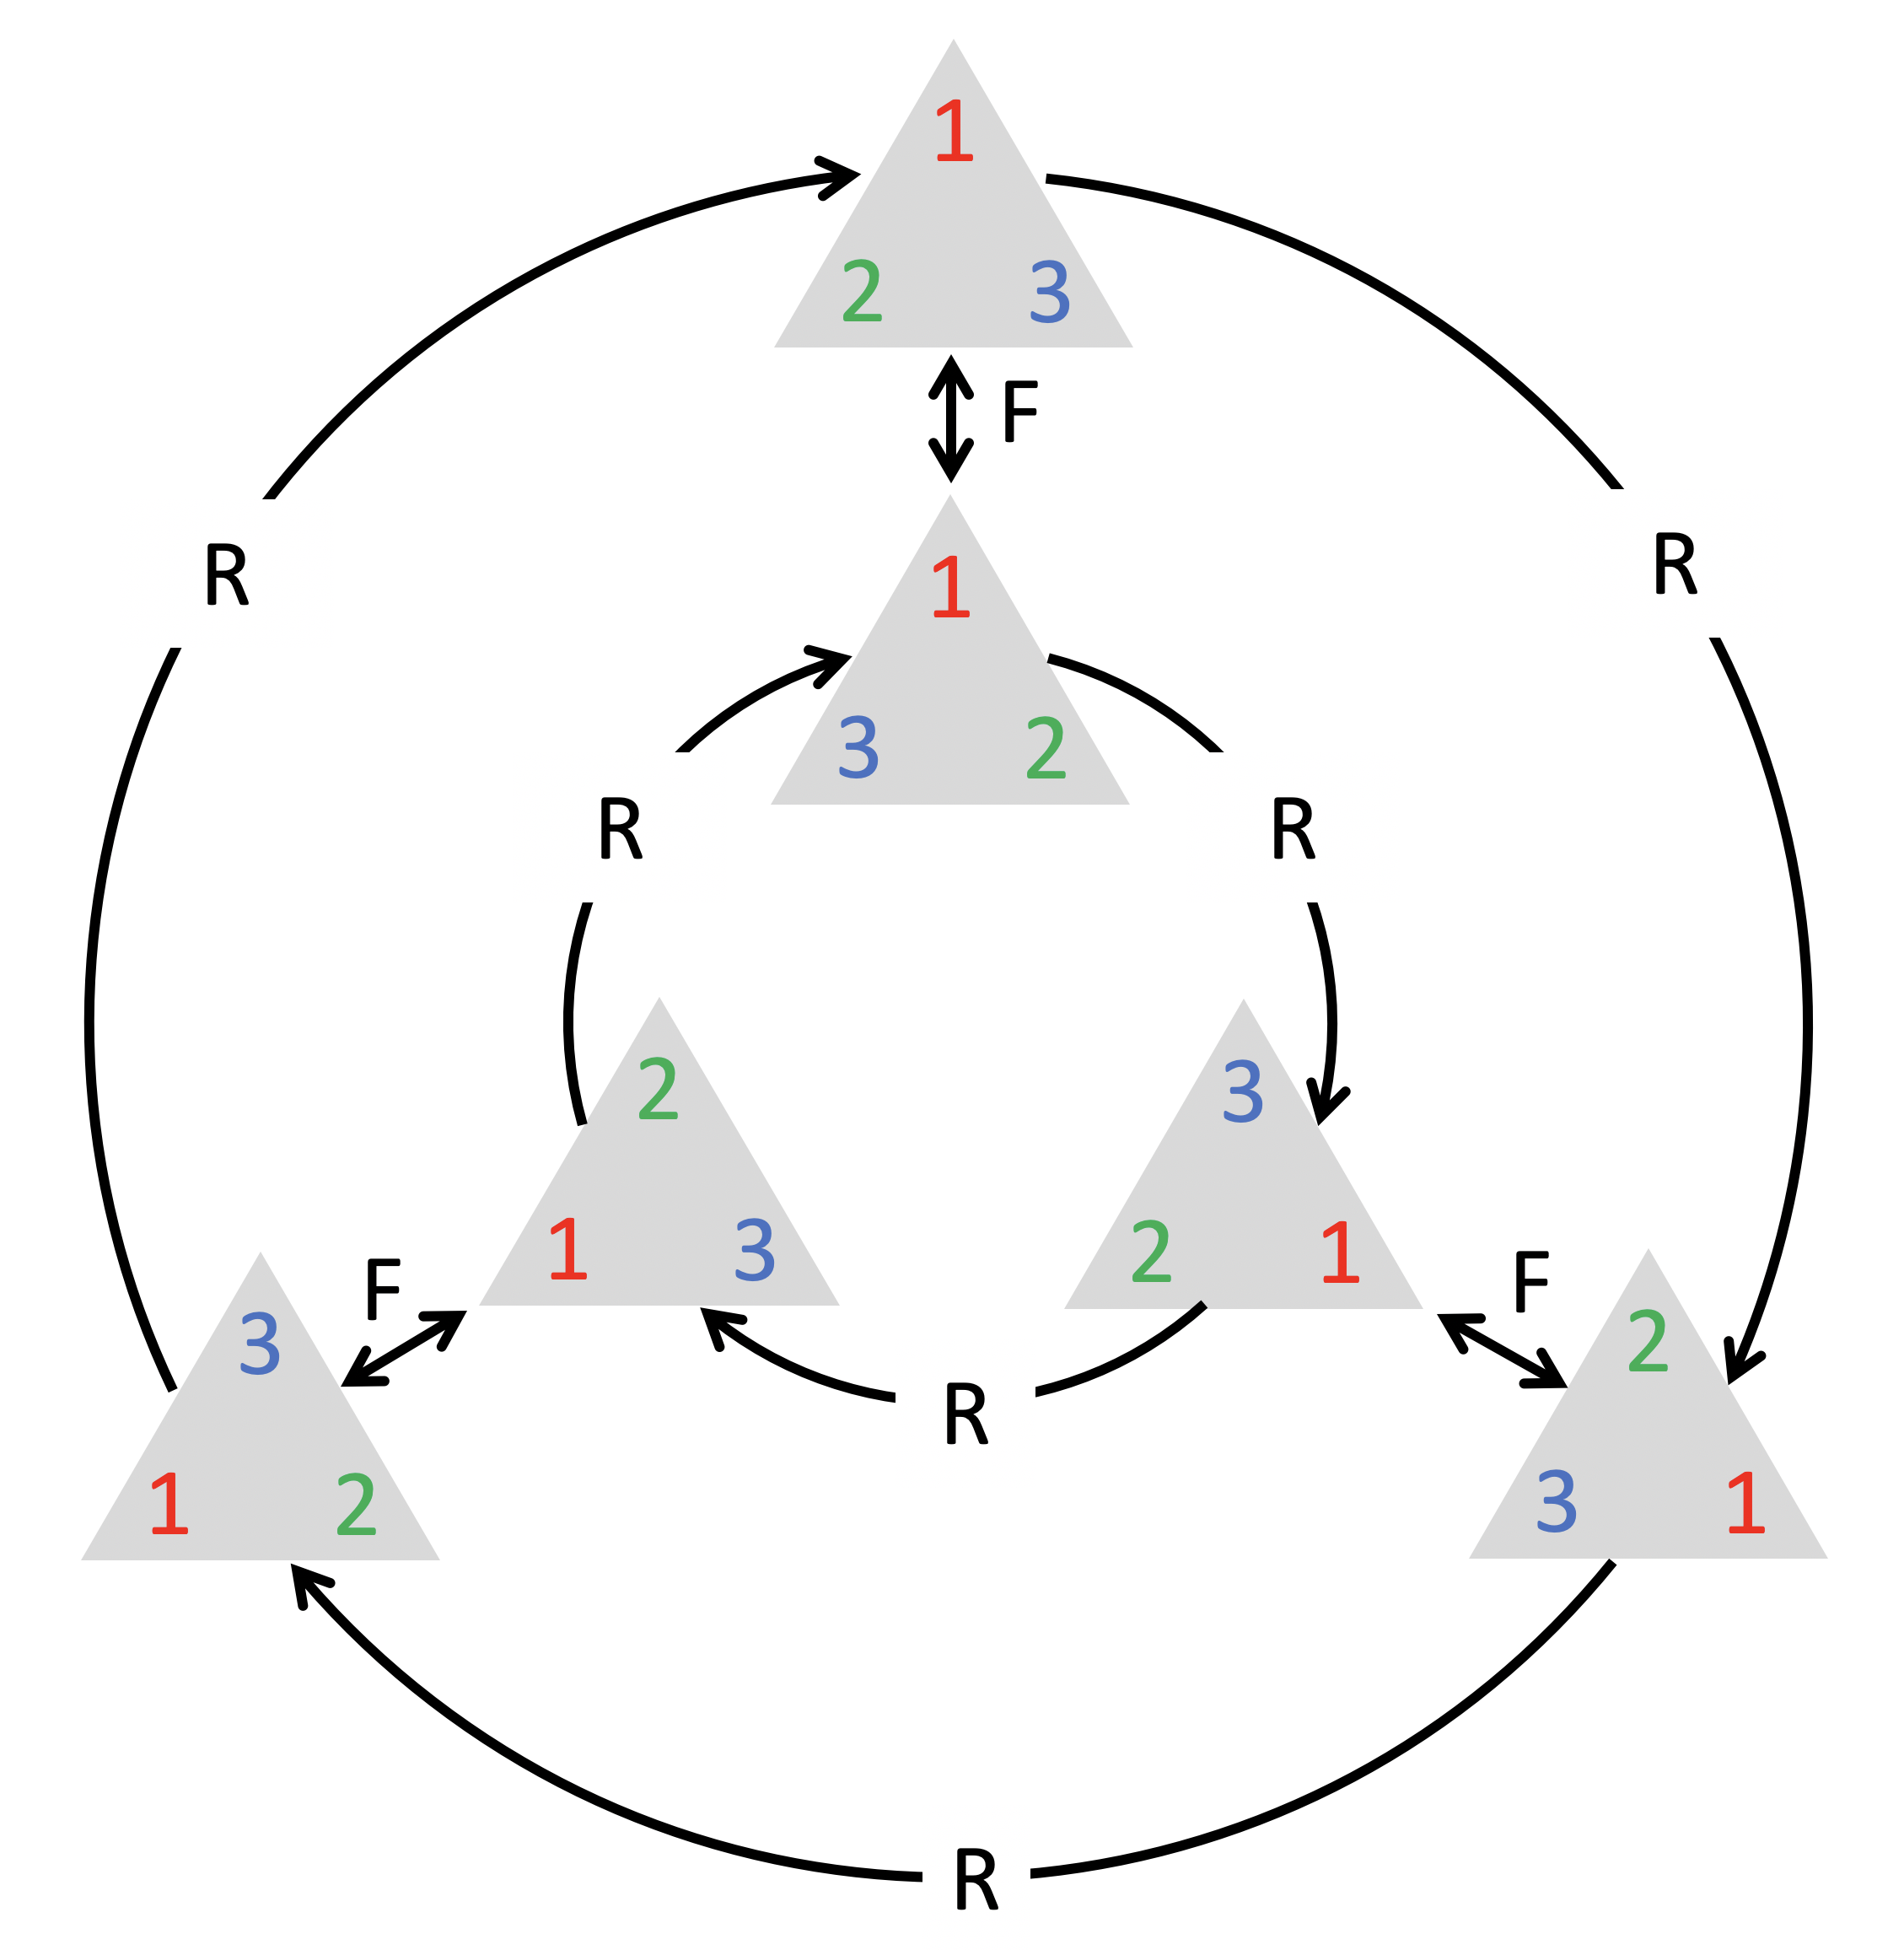
\includegraphics[width=0.45\linewidth]{figures/group_d3.png}
}
    \hspace{2mm}
    \raisebox{-0.5\height}{
        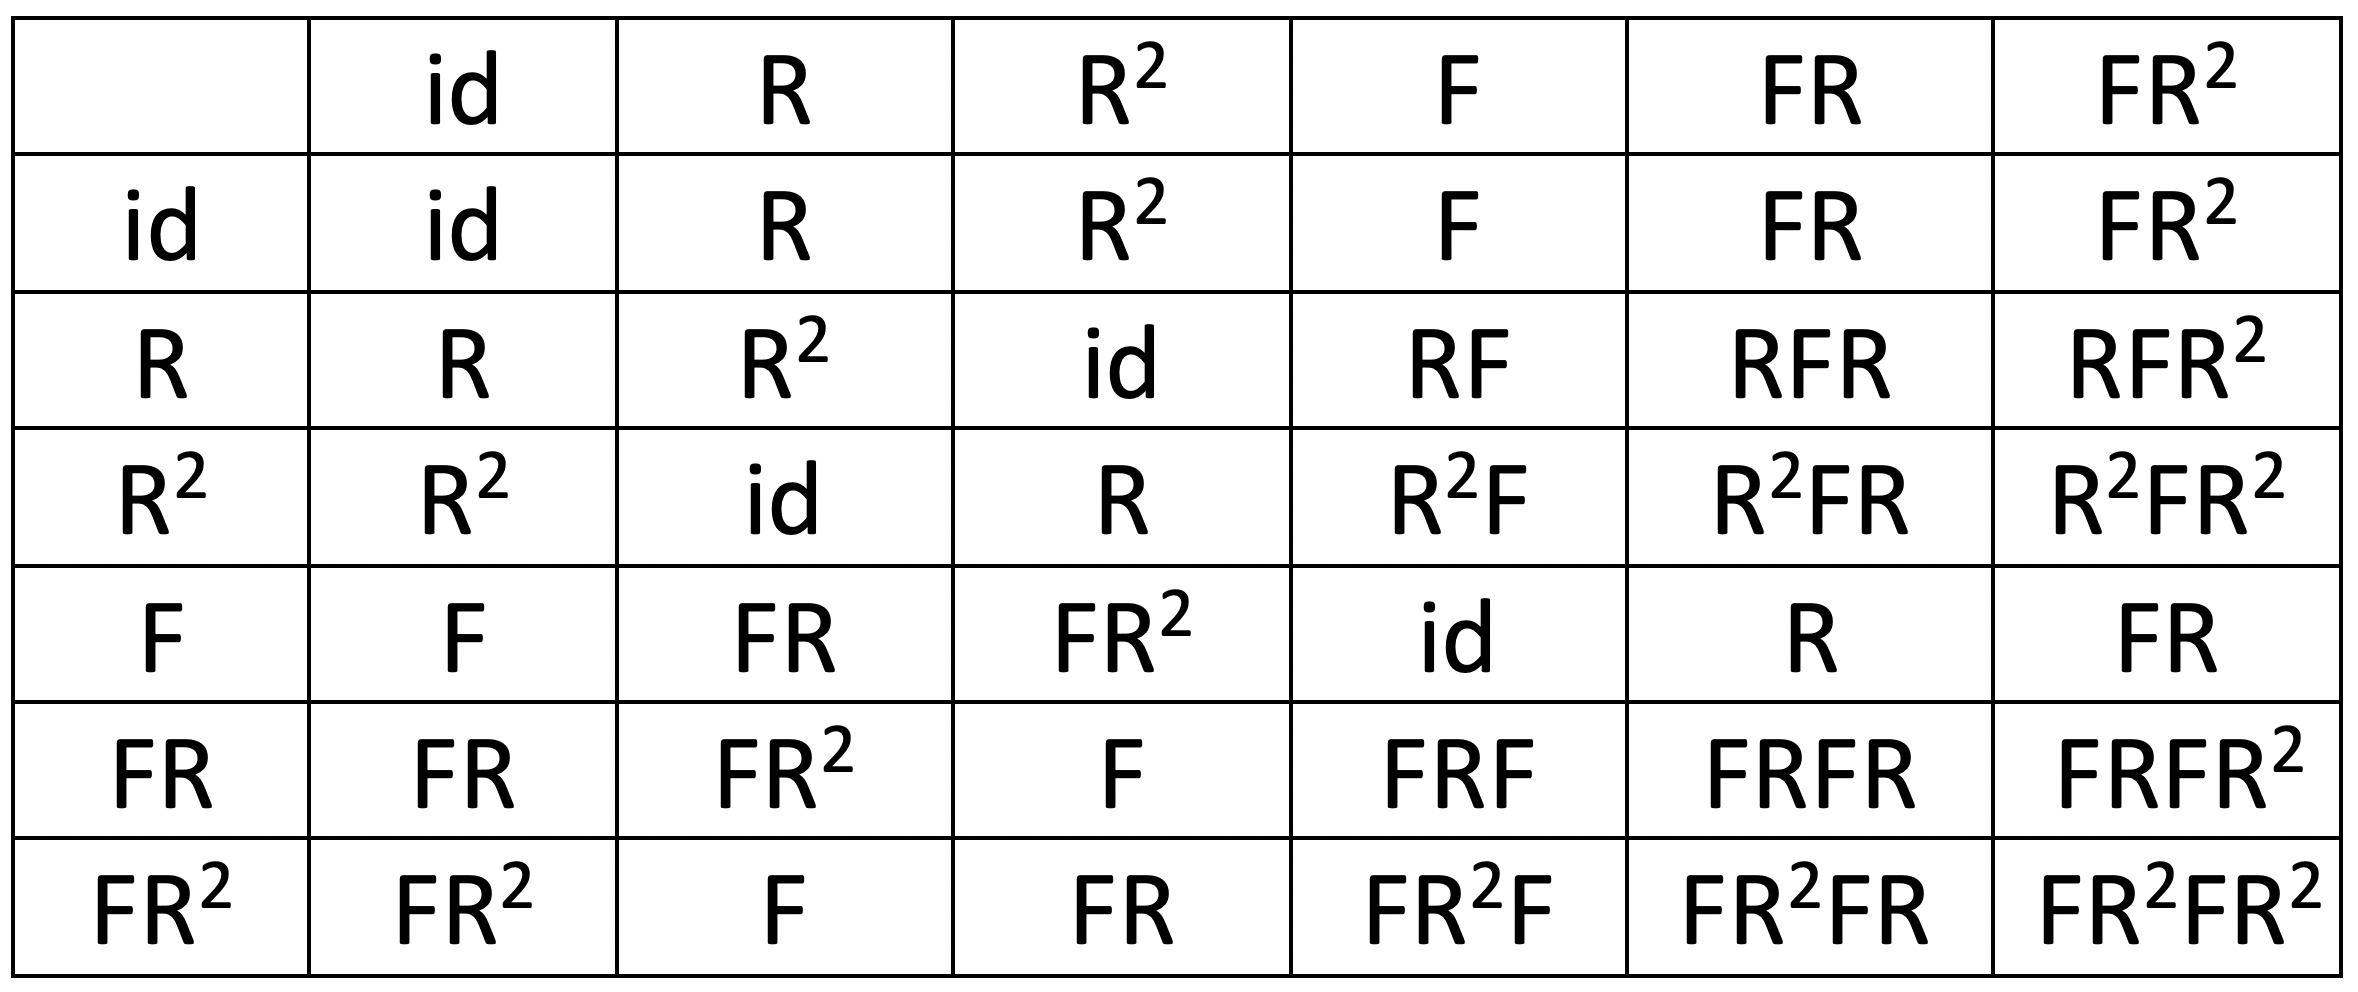
\includegraphics[width=0.48\linewidth]{figures/group_d3_m.png}
        }
%    \taco{TODO: figure of a triangle with labelled corners (0,1,2), and all permutations of it, as a Cayley diagram. Could add multiplication table of the group as well.}
    \caption{Left: an equilateral triangle with corners labelled by $1, 2, 3$, and all possible rotations and reflections of the triangle. The group $\mathrm{D}_3$ of rotation/reflection symmetries of the triangle is generated by only two elements (rotation by $60^\circ$ R and reflection F) and is the same as the group $\Sigma_3$ of permutations of three elements. 
    Right: the multiplication table of the group $\mathrm{D}_3$. The element in the row $\fg$ and column $\fh$ corresponds to the element $\fg \fh$. %\taco{\bf TODO: We need to reverse the Rotation arrows on the outer (or inner) ring. All rotations should be either clockwise or counter-clockwise}}
    \label{fig:group-example-d3-s3}
    }
\end{figure}

% Note that this definition provides a self-consistent description of a standalone object that is the main focus of study in group theory. Despite its apparent simplicity, this theory is rich with many deep results. 
% %despite the apparent simplicity of its basic definition.
% %
% %
% In geometry, key insights are obtained when transformations on a domain are modelled as elements of a group and the group theory formalism is used to study their properties --- this was exactly the breakthrough idea of Klein we have mentioned in the beginning of our discussion. 
% %
% %The way in which elements of symmetry groups act on points on a domain provides important insights about the structure of such domain --- 
% %
% %Group theory is a very rich area with many deep results, despite the apparent simplicity of its basic definition. 
% %
% %symmetry groups turn out to have rich internal algebraic structure with fascinating mathematical properties. 

\paragraph{Group Actions and Group Representations}
%
Rather than considering groups as abstract entities, 
we are mostly interested in how groups \emph{act} on data.
%The structure of such groups reveals the symmetry concealed in the data, which in turn leads to powerful geometric priors. 
%
%The assumption In geometric deep learning, one typically starts 
Since we assumed that there is some domain $\Omega$ underlying our data, we will study how the group acts on $\Omega$ 
(e.g. translation of points of the plane), and from there obtain actions of the same group on the space of signals $\mathcal{X}(\Omega)$
%\marginnote{Whenever possible, we will omit the range $\mathcal{C}$ for brevity.} %in which our data lives 
(e.g. translations of planar images and feature maps). 


% Taco: I am commenting this here, because 1) I think the notion of automorphism should be introduced differently. An auto is an iso from an object to itself. The meaning of iso depends on the context (category), i.e. on what properties/structure we wish to preserve. So when we introduce autos and subgroups, we should just say that we can preserve more or less structure, and get smaller or larger groups. 2) I think here the flow is disrupted a bit, and it would fit better in the deformation section.

% First, let us consider a broad class of bijective domain transformations called {\em automorphisms}
% $$\mathrm{Aut}(\Omega) = \{ \tau: \Omega \xrightarrow{1:1} \Omega \}.$$ 
% %
% Automorphisms also form a group with the composition operation. 
% %
% We can consider symmetries as `subsets' of automorphisms that preserve some structure: for example, in the plane the {\em Euclidean group} $\mathrm{E}(2)$ is the group of transformations of $\R^2$ that preserves Euclidean distances\marginnote{Distance-preserving transformations are called {\em isometries}. According to Klein's Erlangen Programme, the classical Euclidean geometry arises from this group.}, and consists of translations, rotations, and reflections.
% %
% More formally, a symmetry group $\fG$ constitutes a {\em subgroup} of the automorphism group $\mathrm{Aut}(\Omega)$: 

% \begin{tcolorbox}[width=\linewidth,
%                   boxsep=0pt,
%                   left=7.5pt,
%                   right=7.5pt,
%                   top=7.5pt,
%                   bottom=7.5pt,
%                   arc=0pt,
%                   boxrule=0pt,toprule=0pt,
%                   colback=boxgray,
%                   ]%%
% Let $(\fG,\circ)$ be a group and $\mathfrak{H} \subseteq \fG$ a subset. $\mathfrak{H}$ is said to be a {\em subgroup} of $\fG$ if $(\mathfrak{H},\circ)$ constitutes a group with the same operation. 
% \end{tcolorbox}


%we have considered so far are subgroups of $\mathrm{Aut}(\Omega)$. \marginnote{A subset $\fG \subseteq \frak{H}$ is said to be a {\em subgroup} of a group $(\frak{H}, \circ)$ if it forms a group $(\frak{G}, \circ)$ with the same operation.}



%\michael{do we use the . notation? $\fg.u$ of $\fg u$ but $\fg.x$}

A \emph{group action} \marginnote{Technically, what we define here is a {\em left} group action.} of $\fG$ on a set $\Omega$ 
%If $\fG$ is a group of transformations acting on elements of $\Omega$, a \emph{group action}\marginnote{Technically, what we define here is a {\em left} group action, since groups in general are non-commutative. } 
is defined as a mapping $(\fg, u) \mapsto \fg.u$ associating a group element $\fg \in \fG$ and a point $u\in \Omega$ with some other point on $\Omega$ in a way that 
%$(\fg, u) \mapsto \fg.u$
%$(g, x) \in \gG \times \gX \mapsto g.x \in \gX$, 
%that 
is compatible with the group operations, i.e., $\fg.(\fh.u) = (\fg \fh).u$ for all $\fg, \fh \in \fG$ and $u \in \Omega$. 
%
We shall see numerous instances of group actions in the following sections. 
%including translation groups acting on grids or permutation groups acting on sets and graphs.
% TODO: add definition block for group action?
%\michael{\bf [MB: is $g.x$ a standard notation? I suggest $\fg$ as notation for groups]}
%
%Most of the domains we will discuss in this book have some natural symmetries. 
For example, in the plane the {\em Euclidean group} $\mathrm{E}(2)$ is the group of transformations of $\R^2$ that preserves Euclidean distances\marginnote{Distance-preserving transformations are called {\em isometries}. According to Klein's Erlangen Programme, the classical Euclidean geometry arises from this group.}, and consists of translations, rotations, and reflections.
%collection of translation, rotation, and reflection transformations preserving Euclidean distances, so this group acts naturally on the plane.
The same group, however, can also act on the space of \emph{images} on the plane (by translating, rotating and flipping the grid of pixels), as well as on the representation spaces learned by a neural network.
%
%
More precisely, if we have a group $\fG$ acting on $\Omega$, we automatically obtain an action of $\fG$ on the space $\mathcal{X}(\Omega)$: 
%\marginnote{When it is clear from the context, we shall simplify the notation and simply write $\mathcal{X}$ for such space.}
%\michael{Do we need to carry the C here? It is not used; we only need to say that X is a vector space. I suggest to simplify the notation as much as possible. }
\begin{equation}
    (\fg . x)(u) = x(\fg^{-1} u).
    \label{eq:group_action}
\end{equation}
Due to the inverse on $\fg$, this is indeed a valid group action, in that we have $(\fg . (\fh . x))(u) = ((\fg \fh) . x)(u)$.  %(exercise).
%: $(\fg . (\fh . f))(x) = (\fh . f)(\fg^{-1} x) = f(\fh^{-1} \fg^{-1} x) = f((\fg \fh)^{-1} x) = ((\fg \fh). f)(x)$. % leave as exercise?
%\michael{Is this standard notation? Looks abusive to use . for action on $x$ and $u$.}

%
%In our context, the central importance of symmetry groups is due to the fact that they also interact nicely with other less-structured objects. If $\fG$ is a group of transformations acting on elements of some arbitrary set $\gX$, a \emph{group action} is defined as a mapping 
%$(\fg, x) \mapsto \fg.x$
%$(g, x) \in \gG \times \gX \mapsto g.x \in \gX$, 
%that is compatible with the group operations in the sense that $\fg.(\fh.x) = (\fg \circ \fh).x$ for all $\fg, \fh \in \fG$ and $x \in \gX$. We shall see numerous instances of group actions in the next chapters, including translation groups acting on grids or permutation groups acting on sets and graphs.
% TODO: add definition block for group action?
%\michael{\bf [MB: is $g.x$ a standard notation? I suggest $\fg$ as notation for groups]}

The most important kind of group actions, which we will encounter repeatedly throughout this text, are \emph{linear} group actions, also known as {\em group representations}.
The action on signals in equation~(\ref{eq:group_action}) is indeed linear, in the sense that 
$$
\fg . (\alpha x + \beta x') = \alpha (\fg . x) + \beta (\fg . x') $$
%
for any scalars $\alpha, \beta$ and signals $x, x' \in \mathcal{X}(\Omega)$. 
%
We can describe linear actions either as maps $(\fg, x) \mapsto \fg.x$ that are linear in $x$, or equivalently, by currying, 
%\footnote{Currying is the technique of converting a function that takes multiple arguments into a sequence of functions that each take a single argument.}
as a map $\rho : \fG \rightarrow \R^{n \times n}$\marginnote{When $\Omega$ is infinte, the space of signals $\mathcal{X}(\Omega)$ is infinite dimensional, in which case $\rho(\fg)$ is a linear operator on this space, rather than a finite dimensional matrix. In practice, one must always discretise to a finite grid, though.} that assigns to each group element $\fg$ an (invertible) matrix $\rho(\fg)$.
%\michael{Do we want to say representation can be over different space, and here we are interested in the space of signals? We need to say this is a vector space. }
The dimension $n$ of the matrix is in general arbitrary and not necessarily related to the dimensionality of the group or the dimensionality of $\Omega$, but in applications to deep learning $n$ will usually be the dimensionality of the feature space on which the group acts.
For instance, we may have the group of 2D translations acting on a space of images with $n$ pixels.

%\michael{\bf [MB: $n$ has to be defined. This paragraph needs a bit more details/polishing]}
As with a general group action, the assignment of matrices to group elements should be compatible with the group action.
More specifically, the matrix representing a composite group element $\fg \fh$ should equal the matrix product of the representation of $\fg$ and $\fh$:
%\begin{equation}
%    \rho(\fg \fh) = \rho(\fg) \rho(\fh).
%\end{equation}
%\michael{Can we just call this associativity? } \taco{No; both the group operation $\fg \fh$ and the matrix product $\rho(\fg) \rho(\fh)$ are associative, but the equation here says that $\rho$ is a homomorphism. Associativity involves three things being multiplied, $a(bc) = (ab)c$, but here we have two group elements $\fg, \fh$ and one mapping $\rho$, so it's different.}

% History of symmetries in mathematics and physics:
% \begin{itemize}
%     \item Kepler laws of planetary motion. 
%     \item Lagrangian and Hamiltonian of Mechanics invariant to observer frame of reference. 
%     \item Relativity? 
%     \item In mathematics, example of Galois Theory to study the roots of polynomial equations. The structure of such roots is revealed by studying their symmetries. 
% \end{itemize}

\begin{tcolorbox}[width=\linewidth,
                  boxsep=0pt,
                  left=7.5pt,
                  right=7.5pt,
                  top=7.5pt,
                  bottom=7.5pt,
                  arc=0pt,
                  boxrule=0pt,toprule=0pt,
                  colback=boxgray,
                  ]%%
    A $n$-dimensional real \emph{representation} of a group $\fG$ is a map $\rho : \fG \rightarrow \R^{n \times n}$, assigning to each $\fg \in \fG$ an \emph{invertible} matrix $\rho(\fg)$, and satisfying the condition $\rho(\fg \fh) = \rho(\fg) \rho(\fh)$ for all $\fg, \fh \in \fG$.
    \marginnote{Similarly, a complex representation is a map $\rho : \fG \rightarrow \mathbb{C}^{n \times n}$ satisfying the same equation.}
    A representation is called \emph{unitary} or \emph{orthogonal} if the matrix $\rho(\fg)$ is unitary or orthogonal for all $\fg \in \fG$.
\end{tcolorbox}

Written in the language of group representations, the action of $\fG$ on signals $x \in \mathcal{X}(\Omega)$ is defined as $\rho(\fg) x(u) = x(\fg^{-1} u)$.
%
We again verify that 
$$
(\rho(\fg) (\rho(\fh) x))(u) = (\rho(\fg \fh) x)(u).
$$
%



% Removing stuff on subgroups and homogeneous spaces, as we don't really need it to talk about groups, representations and equivariance.
% % Consider moving this right after the definition of group, since the notion of subgroup does not rely on the notion of group action... 
% A subset of a group that is itself a group (i.e. is closed under composition and inverses, and contains the identity) is called a \emph{subgroup}.
% For example, the group $\mathrm{E}(2)$ contains the subset of rotations and translations (also called `roto-translations'), which is closed under composition and forms a group called the {\em special Euclidean group} $\SE{2}$. Finally, translations by themselves form the {\em translation group}. 
% %


% The plane is an example of a space in which ``all points are the same'', in the sense that one point can be transformed into another by means of a symmetry. 
% %
% Such a space is said to be {\em homogeneous} and requires that for any two points $u, v \in \Omega$ there is $\fg \in \fG$ such that $u = \fg v$. 
% %or in other words, one point can be transformed into another by means of a symmetry. 


\begin{figure}
    \centering
    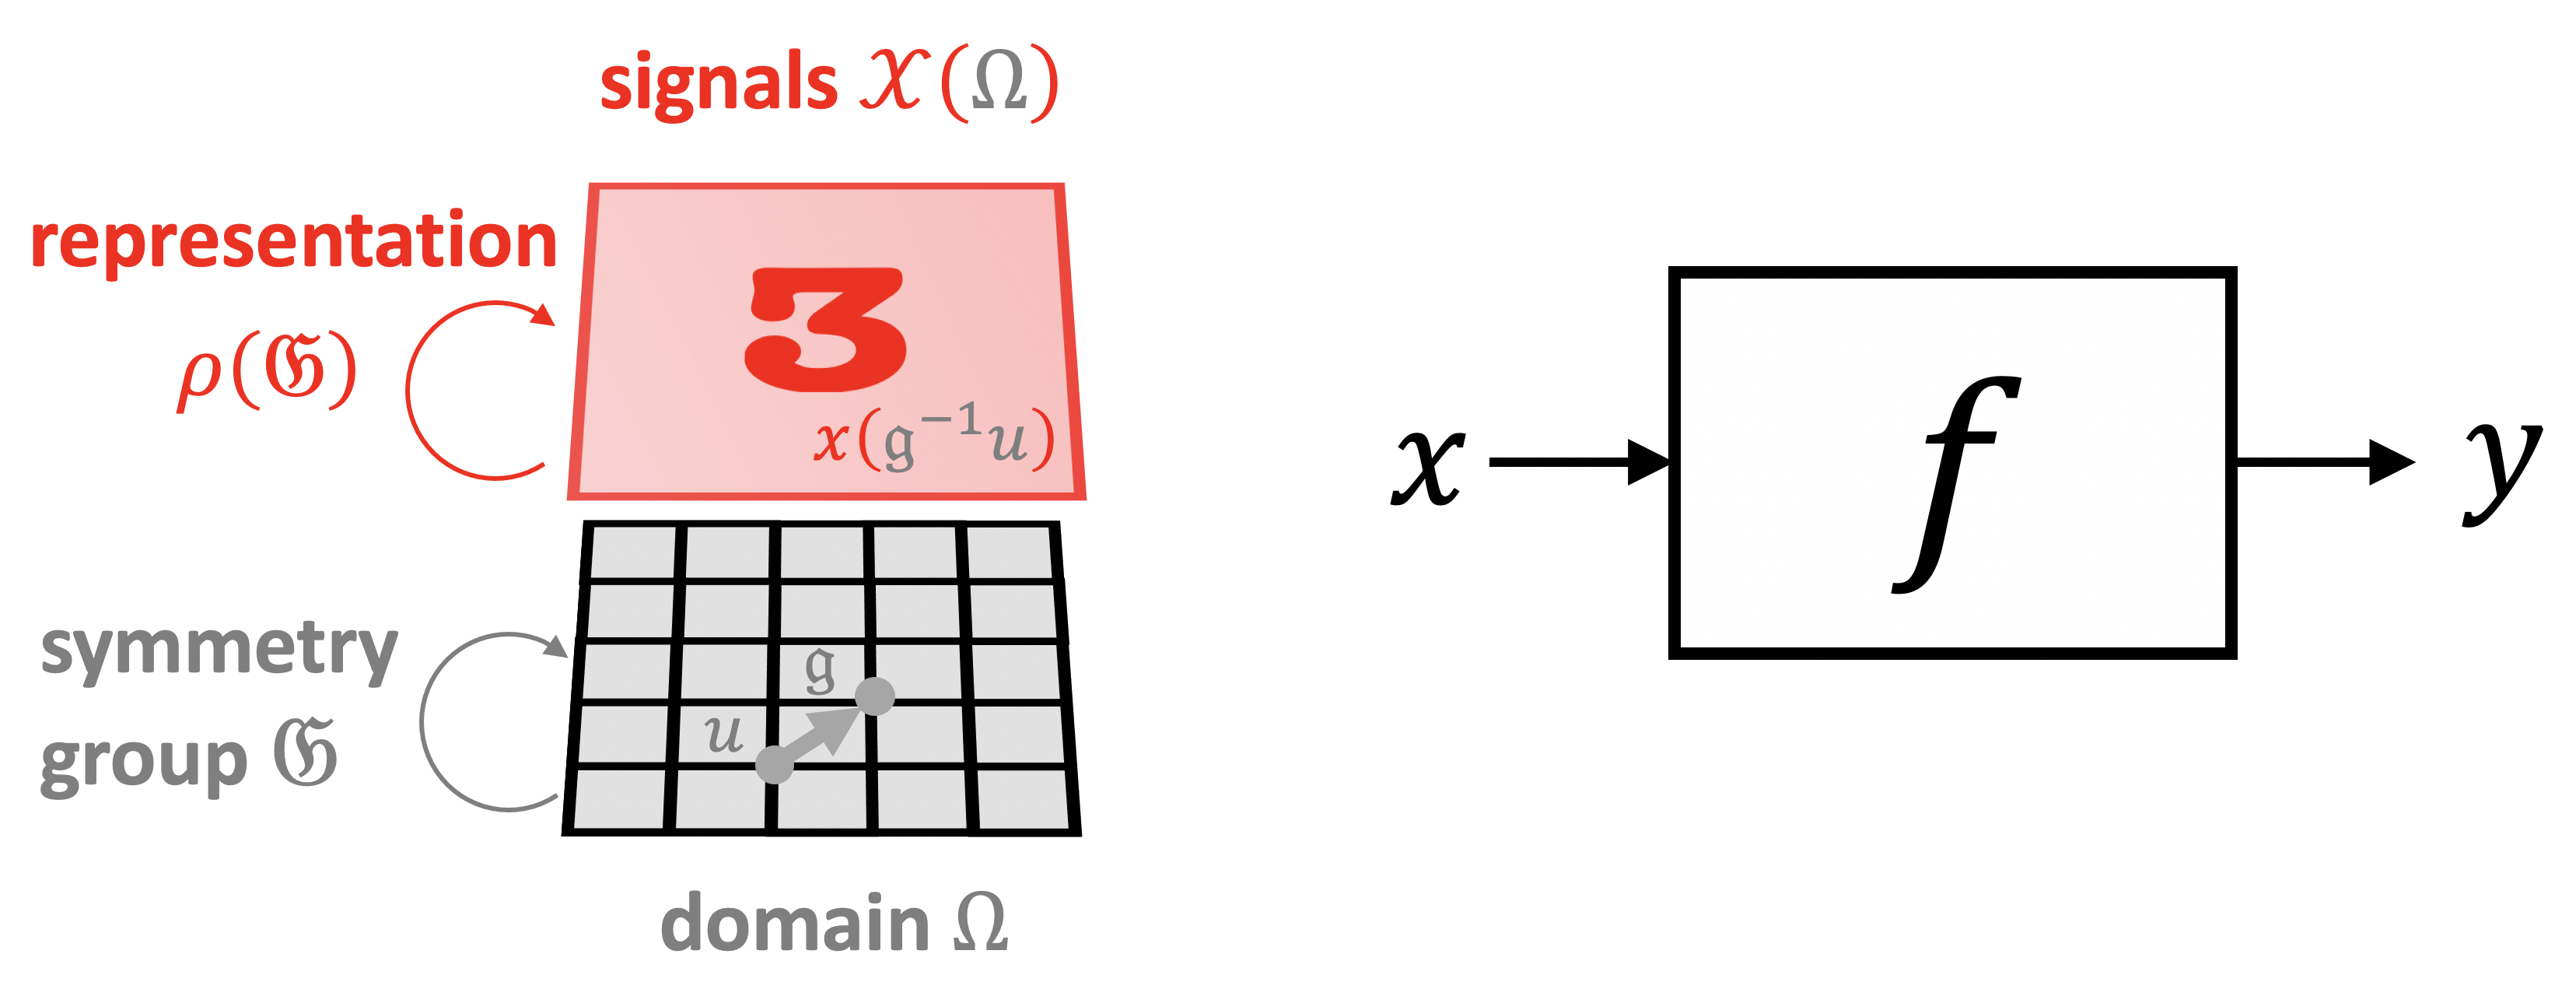
\includegraphics[width=0.75\linewidth]{figures/geom_prior.png}%groups1.pdf}
    \caption{
    Three spaces of interest in Geometric Deep Learning: the (physical) {\em domain} $\Omega$, the space of {\em signals} $\mathcal{X}(\Omega)$, and the {\em hypothesis} class $\mathcal{F}(\mathcal{X}(\Omega))$. 
    %
    Symmetries of the domain $\Omega$ (captured by the group $\fG$) act on signals $x\in \mathcal{X}(\Omega)$ through group representations $\rho(\fg)$, imposing structure on the functions $f\in \mathcal{F}(\mathcal{X}(\Omega))$ acting on such signals.
    }
    \label{fig:symmetryactors}
\end{figure}


\paragraph{Invariant and Equivariant functions}

The symmetry of the domain $\Omega$ underlying the signals $\mathcal{X}(\Omega)$ imposes structure on the function $f$ defined on such signals. 
%
It turns out to be a powerful inductive bias, improving learning\marginnote{In general, $f$ depends both on the signal an the domain, i.e., $\mathcal{F}(\mathcal{X}(\Omega), \Omega)$. We will often omit the latter dependency for brevity. } efficiency by reducing the space of possible interpolants, $\mathcal{F}(\mathcal{X}(\Omega))$, to those which satisfy the symmetry priors. 
%
%Adding such known symmetries into the function hypothesis class of a machine learning system is a powerful inductive bias, improving learning efficiency by reducing the space of possible interpolants to those which satisfy the symmetry priors. 
%
Two important cases we will be exploring in this text are {\em invariant} and {\em equivariant} functions. 


%is its output is unaffected by the action of the group on the argument


\begin{tcolorbox}[width=\linewidth,
                  boxsep=0pt,
                  left=7.5pt,
                  right=7.5pt,
                  top=7.5pt,
                  bottom=7.5pt,
                  arc=0pt,
                  boxrule=0pt,toprule=0pt,
                  colback=boxgray,
                  ]%%
    A function $f: \mathcal{X}(\Omega) \rightarrow \mathcal{Y}$ is $\fG$-{\em invariant} if 
    $
    f(\rho(\fg)x) = f(x)$  for all $\fg \in \fG$ and $x \in \mathcal{X}(\Omega)$, i.e., its output is unaffected by the group action on the input. 
\end{tcolorbox}


A classical example of invariance is {\em shift-invariance},\marginnote{Note that signal processing books routinely use the term `shift-invariance' referring to shift-equivariance, e.g. Linear Shift-invariant Systems. } 
arising in computer vision and pattern recognition applications such as image classification. The function $f$ in this case (typically implemented as a Convolutional Neural Network) inputs an image and outputs the probability of the image to contain an object from a certain class (e.g. cat or dog). %
%
It is often reasonably assumed that the classification result should not be affected by the position of the object in the image, i.e., the function $f$ must be shift-invariant. 
%
Multi-layer Perceptrons, which can approximate any smooth function, do not have this property -- one of the reasons why early attempts to apply these architectures to problems of pattern recognition in the 1970s failed. 
%
The development of neural network architectures with local weight sharing, as epitomised by Convolutional Neural Networks, was, among other reasons, motivated by the need for shift-invariant object classification. 


If we however take a closer look at the convolutional layers of CNNs, we will find that they are not shift-invariant but {\em shift-equivariant}: in other words, a shift of the input to a convolutional layer produces a shift in the output feature maps by the same amount. 

\begin{tcolorbox}[width=\linewidth,
                  boxsep=0pt,
                  left=7.5pt,
                  right=7.5pt,
                  top=7.5pt,
                  bottom=7.5pt,
                  arc=0pt,
                  boxrule=0pt,toprule=0pt,
                  colback=boxgray,
                  ]%%
    A function $f: \mathcal{X}(\Omega) \rightarrow \mathcal{X}(\Omega)$ is $\fG$-{\em equivariant} if\marginnote{
    More generally, we might have $f: \mathcal{X}(\Omega) \rightarrow \mathcal{X}(\Omega')$ with input and output spaces having different domains $\Omega, \Omega'$ and representations $\rho$, $\rho'$ of the same group $\fG$.
    In this case, equivariance is defined as $f(\rho(\fg)x) = \rho'(\fg) f(x)$.
    %symmetry groups, $\fG$ and $\fG'$. In this case, equivariance is defined as $ f(\rho(\fg)x) = \rho'(\fg) f(x)$, where $\rho'$ is the representation of $\fG'$.
    } 
    $f(\rho(\fg)x) = \rho(\fg) f(x)$  for all $\fg \in \fG$, i.e., group action on the input affects the output in the same way. 
\end{tcolorbox}




Resorting again to computer vision, a prototypical application requiring shift-equivariance is image segmentation, where the output of $f$ is a pixel-wise image mask. 
%
Obviously, the segmentation mask must follow shifts in the input image.  
In this example, the domains of the input and output are the same, but since the input has three color channels while the output has one channel per class, the representations $(\rho, \mathcal{X}(\Omega, \mathcal{C}))$ and $(\rho', \mathcal{X}(\Omega, \mathcal{C}'))$ are somewhat different.


However, even the previous use case of image classification is usually implemented as a sequence of convolutional (shift-equivariant) layers, followed by global pooling (which is shift-invariant). 
%
As we will see in Section~\ref{sec:gdl_blueprint}, this is a general blueprint of a majority of deep learning architectures, including CNNs and Graph Neural Networks (GNNs). 
%: a sequence of equivariant layers, optionally followed by invariant layers. 


%In supervised learning, the goal is to approximate some function $f : \mathcal{X} \rightarrow \mathcal{X}'$ from a finite set of samples.
%In many cases, the problem has symmetries, which means that $f$ is either invariant ($f(\rho(\fg) x) = f(x)$ for all $\fg \in \fG$) or equivariant ($f(\rho(\fg) x) = \rho'(\fg) f(x)$).
%For instance, in image classification the class label is invariant, whereas the segmentation mask is equivariant. 
% In machine learning, where one tries to approximate some unknown function $f$ from a finite set of samples, $f$ often has known symmetries.
% Canonical examples include translations in computer vision and image classification tasks, rotations in molecular prediction problems, or permutations in 3D graphics point-cloud processing tasks. 
% %
% In such settings, given some domain $\gX$ with a certain symmetry group $\fG$, we say that 
% $f: \gX \to \gY$ is $\fG$\emph{-invariant} if $f(\fg.x) = f(x)$ for all $x\in \gX$ and $\fg \in \fG$. If in addition $\fG$ is also acting on $\gY$, we say that $f$ is $\fG$\emph{-equivariant} if $f(\fg.x) = \fg.(f(x))$.
% % We will explore these concepts in detail in Chapter ??. 
%Adding such known symmetries into the function hypothesis class %$\gF$ 
%of a machine learning system is a powerful inductive bias, improving learning efficiency by reducing the space of possible interpolants to those which satisfy the symmetry priors. 


% Possible todo's for this section:
% Explain in/equivariance mathematically (at a high level only)
% Explain group representations (idem)


%\taco{TODO: add definition of space of signals, and regular rep acting on it}

%\taco{TODO: Figure showing domain Omega, group action of G on Omega, and the space of functions X on Omega}

\subsection{Isomorphisms and Automorphisms}
\label{sec:isomorphism}

\paragraph{Subgroups and Levels of structure}

As mentioned before, a symmetry\marginnote{Invertible and structure-preserving maps between different objects often go under the generic name of {\em isomorphisms} (Greek for `equal shape'). An isomorphism from an object to itself is called an {\em automorphism}, or symmetry.}
%We will mainly use this term for maps preserving the connectivity of graphs.}
is a transformation that preserves some property or structure, and the set of all such transformations for a given structure forms a symmetry group.
It happens often that there is not one but multiple structures of interest, and so we can consider several {\em levels of structure} on our domain $\Omega$. 
%
%We can thus formalise symmetries as invertible maps $\tau: \Omega \rightarrow \Omega$ that preserve some structure. % and satisfy the group axioms with the function composition operation.  
Hence, what counts as a symmetry depends on the structure under consideration, but in all cases a symmetry is an invertible map that respects this structure.

On the most basic level, the domain $\Omega$ is a \emph{set}, which has a minimal amount of structure: all we can say is that the set has some \emph{cardinality}\marginnote{For a finite set, the cardinality is the number of elements (`size') of the set, and for infinite sets the cardinality indicates different kinds of infinities, such as the countable infinity of the natural numbers, or the uncountable infinity of the continuum $\R$.}. %, and which elements are members of the set.
Self-maps that preserve this structure are  \emph{bijections} (invertible maps), which we may consider as set-level symmetries.
%A more formal way to say the same is that the automorphism group $\mathrm{Aut}(\Omega)$ in the category of sets is the group of bijections $\tau : \Omega \rightarrow \Omega$.
%Such maps are often referred to as (set-){\em automorphisms} and denoted by $\mathrm{Aut}(\Omega)$. 
%
One can easily verify that this is a group by checking the axioms: a compositions of two bijections is also a bijection (closure), the associativity stems from the associativity of the function composition, the map $\tau(u)=u$ is the identity element, and for every $\tau$ the inverse exists by definition, satisfying $(\tau \circ \tau^{-1})(u) = (\tau^{-1} \circ \tau)(u) =u$.


Depending on the application, there may be further levels of structure.  
%
For instance, if $\Omega$ is a topological space, we can consider maps that preserve {\em continuity}: such maps are called {\em homeomorphisms} and in addition to simple bijections between sets, are also continuous and have continuous inverse.  
%
Intuitively, continuous functions are well-behaved and map points in a neighbourhood (open set) around a point $u$ to a neighbourhood around $\tau(u)$.  
%Thus, homeomorphisms $\tau : \Omega \rightarrow \Omega$ are the automorphisms / symmetries of $\Omega$ viewed as a topological space.


%
%
One can further demand that the map and its inverse are (continuously) {\em  differentiable},\marginnote{Every differentiable function is continuous. If the map is continuously differentiable `sufficiently many times', it is said to be {\em smooth}.} i.e., the map and its inverse have a derivative at every point (and the derivative is also continuous). 
%
This requires further differentiable structure that comes with differentiable manifolds, where such maps are called {\em diffeomorphisms} and denoted by $\mathrm{Diff}(\Omega)$. 
%These are the automorphisms of smooth manifolds.
%
%
Additional examples of structures we will encounter include {\em distances} or {\em metrics} (maps preserving them are called {\em isometries}) or {\em orientation} (to the best of our knowledge, orientation-preserving maps do not have a common Greek name). 


\begin{tcolorbox}[width=\linewidth,
                  boxsep=0pt,
                  left=7.5pt,
                  right=7.5pt,
                  top=7.5pt,
                  bottom=7.5pt,
                  arc=0pt,
                  boxrule=0pt,toprule=0pt,
                  colback=boxgray,
                  ]%%
A {\em metric} or {\em distance} is a function $d:\Omega\times\Omega \rightarrow [0,\infty)$ satisfying for all $u,v,w \in \Omega$:  \vspace{3mm}\\
%\begin{enumerate}
    %\item 
    \noindent {\em 	Identity of indiscernibles:} $d(u,v) =0$ iff $u=v$.\vspace{2mm}\\
    \noindent  {\em Symmetry:} $d(u,v) = d(v,u)$.\vspace{2mm}\\
    \noindent  {\em Triangle inequality:} $d(u,v) \leq  d(u,w) + d(w,v)$.\vspace{2mm}\\
%\end{enumerate}

A space equipped with a metric $(\Omega,d)$ is called a {\em metric space}. 

\end{tcolorbox}




%an image plane can be viewed as a smooth manifold, in which case any smooth deformation (diffeomorphism) should be considered a symmetry.
%In practice the object identity will not be preserved by arbitrarily large deformations, so we may add a distance metric, i.e. view the image plane as a Riemannian manifold, in which case only distance-preserving transformations (isometries) can be considered as symmetries.
%As a further example, independently of whether we care about distances, we can assign an \emph{orientation} to the plane, i.e. clockwise or counterclockwise, and consider only orientation-preserving transformations.

The right level of structure to consider depends on the problem.
For example, when segmenting histopathology slide images, we may wish to consider flipped versions of an image as equivalent (as the sample can be flipped when put under the microscope), but if we are trying to classify road signs, we would only want to consider orientation-preserving transformations as symmetries (since reflections could change the meaning of the sign).
%{\bf [Figure?]}

As we add levels of structure to be preserved, the symmetry group will get smaller.
Indeed, adding structure is equivalent to selecting a \emph{subgroup}, which is a subset of the larger group that satisfies the axioms of a group by itself:  
%(i.e. it is closed under composition and inverses, and contains the identity).
 
 \begin{tcolorbox}[width=\linewidth,
                   boxsep=0pt,
                   left=7.5pt,
                   right=7.5pt,
                   top=7.5pt,
                   bottom=7.5pt,
                   arc=0pt,
                   boxrule=0pt,toprule=0pt,
                   colback=boxgray,
                   ]%%
 Let $(\fG,\circ)$ be a group and $\mathfrak{H} \subseteq \fG$ a subset. $\mathfrak{H}$ is said to be a {\em subgroup} of $\fG$ if $(\mathfrak{H},\circ)$ constitutes a group with the same operation. 
 \end{tcolorbox}
 
For instance, the group of Euclidean isometries $\E{2}$ is a subgroup of the group of planar diffeomorphisms $\diff{2}$, and in turn the group of orientation-preserving isometries $\SE{2}$ is a subgroup of $\E{2}$.
This hierarchy of structure follows the Erlangen Programme philosophy outlined in the Preface: in Klein's construction, the Projective, Affine, and Euclidean geometries have increasingly more invariants and correspond to progressively smaller groups. 


\paragraph{Isomorphisms and Automorphisms}
% Optional: discuss the notion of isomorphic objects, and present symmetries as self-isomorphisms i.e. automorphisms. Thus the notion of symmetry depends on the notion of iso, i.e. the category we're working in, i.e. the level of structure as discussed above.

We have described symmetries as structure preserving and invertible maps \emph{from an object to itself}.
Such maps are also known as \emph{automorphisms}, and describe a way in which an object is equivalent it itself.
However, an equally important class of maps are the so-called \emph{isomorphisms}, which exhibit an equivalence between two non-identical objects.
These concepts are often conflated, but distinguishing them is necessary to create  clarity for our following discussion.

To understand the difference, consider a set $\Omega = \{0,1,2\}$.
An automorphism of the set $\Omega$ is a bijection $\tau : \Omega \rightarrow \Omega$ such as a cyclic shift $\tau(u) = u + 1 \mod 3$.
Such a map preserves the cardinality property, and maps $\Omega$ onto itself.
If we have another set $\Omega' = \{a, b, c\}$ with the same number of elements, then a bijection $\eta : \Omega \rightarrow \Omega'$ such as $\eta(0) = a$, $\eta(1) = b$, $\eta(2) = c$ is a {\em set isomorphism}.

As we will see in Section~\ref{sec:proto-graphs}
for graphs, %$\Omega$, 
the notion of structure includes not just the number of nodes, but also the connectivity.
An isomorphism $\eta: \mathcal{V} \rightarrow \mathcal{V}'$ between two graphs $\mathcal{G}=(\mathcal{V},\mathcal{E})$ and $\mathcal{G}'=(\mathcal{V}',\mathcal{E}')$ is thus a bijection between the nodes that maps pairs of connected nodes to pairs of connected nodes, and likewise for pairs of non-connected nodes.\marginnote{I.e., $(\eta(u),\eta(v)) \in \mathcal{V}'$ iff $(u,v) \in \mathcal{V}$. } Two isomorphic graphs are thus structurally identical, and differ only in the way their nodes are ordered. \marginnote{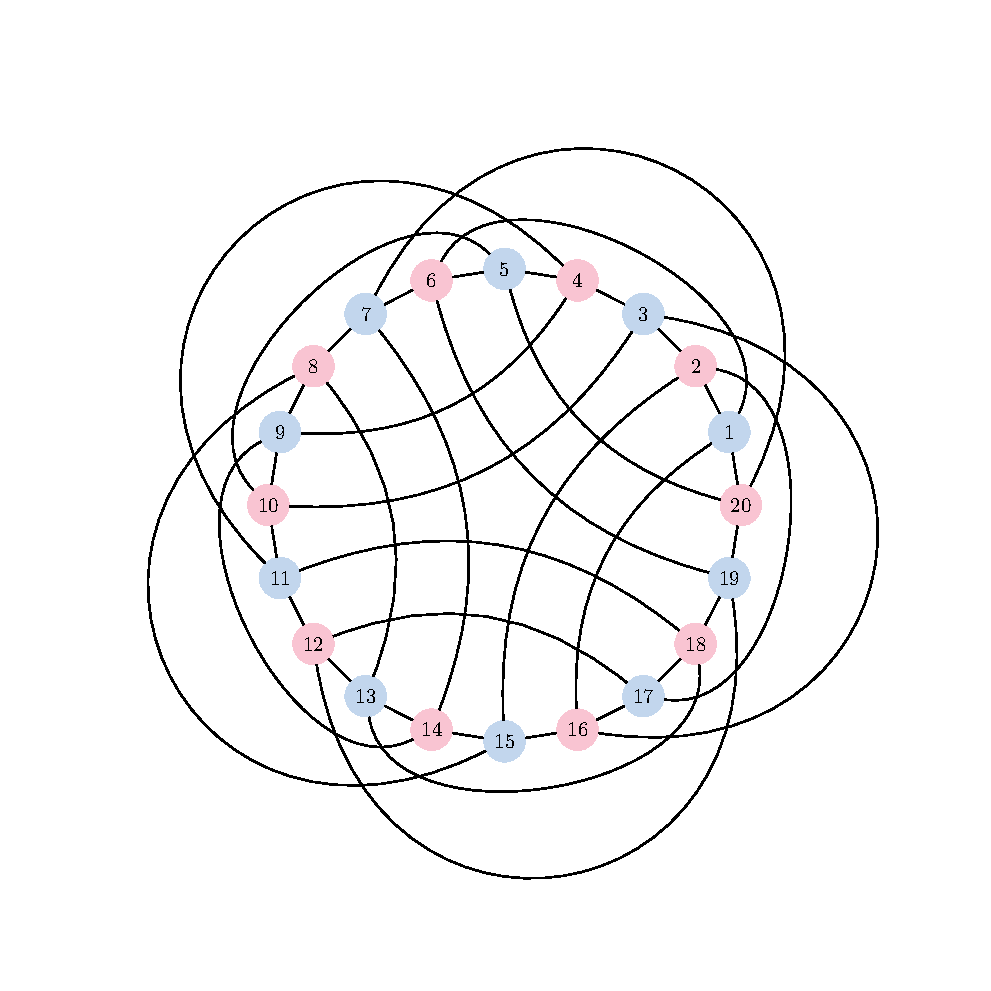
\includegraphics[width=\linewidth]{figures/folkman_g.pdf}\vspace{-2mm}\\ The \emph{Folkman graph} \citep{folkman1967regular} is a beautiful example of a graph with 3840  automorphisms, exemplified by the many symmetric ways to draw it.}
%
On the other hand, a graph automorphism or symmetry is a map $\tau : \mathcal{V} \rightarrow \mathcal{V}$ maps the nodes of the graph back to itself, while preserving the connectivity. A graph with a non-trivial automorphism (i.e., $\tau \neq \mathrm{id}$) presents symmetries.
%\michael{Show in a figure}

%An isomorphism of graphs is thus not the same as a symmetry, but it is just as important that our neural network treat isomorphic objects equivalently.
% when we're dealing with isos vs autos. Example of sphere and graph

% same number of isos A -> B and autos A -> A. Isomorphic objects have isomorphic automorphism groups




\subsection{Deformation Stability}
\label{sec:geom_stab}
%While the Fourier representation is useful to represent {\em signals} $\gX(\Omega)$ on a domain $\Omega$, it is not necessarily useful to regularise the space of {\em functions on such signals}, $\mathcal{F}(\mathcal{X}(\Omega))$ used in supervised learning problems. 
%
%Despite its far-reaching implications, the Fourier representation $\hat{x}$ is not necessarily useful to regularise the space of functions $\{ f : \gX \to \gY \}$, 
%the ultimate goal of supervised learning. 
%
The symmetry formalism introduced in Sections~\ref{sec:symmetries}--\ref{sec:isomorphism} captures an idealised world where we know exactly which transformations are to be considered as symmetries, and we want to respect these symmetries {\em exactly}. 
%the transformations affecting the input are captured with simple mathematical models.
For instance in computer vision, we might assume that planar translations are exact symmetries.
%model for input variability parametrised by only two degrees of freedom (the translations in the plane). 
However, the real world is noisy and this model falls short in two ways. %: it only describes \emph{global} transformations, and 

\marginnote{
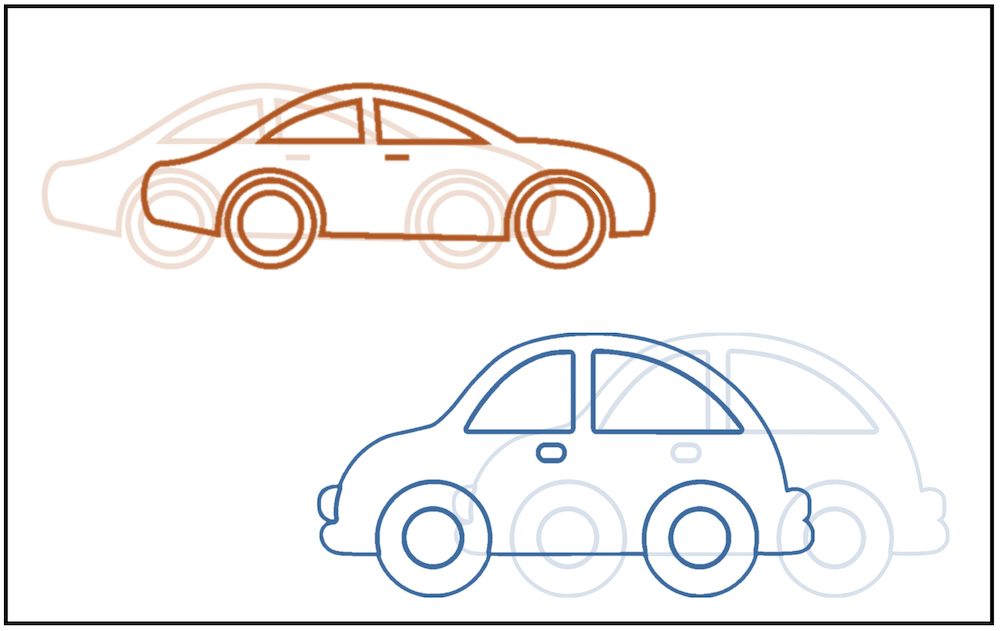
\includegraphics[width=0.95\linewidth]{figures/videosketch.png}
Two objects moving at different velocities in a video define 
a transformation outside the translation group.
}
Firstly, while these simple groups provide a way to understand \emph{global} symmetries of the domain $\Omega$ (and by extension, of signals on it, $\gX(\Omega)$), they do not capture \emph{local} symmetries well. 
%
For instance, consider a video scene %$x=x_t$ 
with several objects, each moving along its own different direction.
At subsequent frames, the resulting scene 
%$x_{t+\delta t}$ 
will contain approximately the same semantic information, yet no global translation explains the transformation from one frame to another.
In other cases, such as a deformable 3D object viewed by a camera, it is simply very hard to describe the group of transformations that preserve the object identity.
These examples illustrate that in reality we are more interested in a %beneath the global symmetry group lies a 
far larger set of transformations where global, exact invariance is replaced by a local, inexact one.
%
In our discussion, we will distinguish between two scenarios: the setting where the domain $\Omega$ is fixed, and signals $x \in \gX(\Omega)$ are undergoing deformations, and the setting where the domain $\Omega$ itself may be deformed.
%\taco{TODO: perhaps move this up, and discuss this as isomorphisms vs automorphisms?}

%In the language of group representations, we thus need to account for a broader class of bijective domain transformations called {\em automorphisms}, $\mathrm{Aut}(\Omega) = \{ \tau: \Omega \xrightarrow{1:1} \Omega \}$. 
\paragraph{Stability to signal deformations}
In many applications, we know a priori that a small deformation of the signal $x$ should not change the output of $f(x)$, so it is tempting to consider such deformations as symmetries.
For instance, we could view small diffeomorphisms $\tau \in \diff{\Omega}$, or even small bijections, as symmetries.
However, small deformations can be composed to form large deformations, so ``small deformations'' do not form a group,\marginnote{E.g., the composition of two $\epsilon$-isometries is a $2\epsilon$-isometry, violating the closure property. } and we cannot ask for invariance or equivariance to small deformations only.
Since large deformations can can actually materially change the semantic content of the input, it is not a good idea to use the full group $\diff{\Omega}$ as symmetry group either.

A better approach is to quantify how ``far'' a given $\tau \in \diff{\Omega}$ is from a given symmetry subgroup $\fG \subset \diff{\Omega}$ (e.g. translations)
with a complexity measure $c(\tau)$, so that $c(\tau) = 0$ whenever $\tau \in \fG$. 
We can now replace our previous  definition of exact invariance and equivarance under group actions with a `softer' notion of  
\emph{deformation stability} (or {\em approximate invariance}):
\begin{equation}
\label{eq:defstability1}
\| f(\rho(\tau) x) - f(x)\| \leq C c(\tau) \|x\|,~,~    \forall x\in \gX(\Omega)
\end{equation}
where $\rho(\tau)x(u) = x(\tau^{-1} u)$ as before, and where $C$ is some constant independent of the signal $x$. 
A function $f\in \mathcal{F}(\mathcal{X}(\Omega))$ satisfying the above equation is said to be {\em geometrically stable}. 
%
We will see examples of such functions in the next Section~\ref{sec:scale_separation}. 


Since $c(\tau)=0$ for $\tau \in \fG$, this definition generalises the $\fG$-invariance property defined above. Its utility in applications depends on introducing an appropriate deformation cost. In the case of images defined over a continuous Euclidean plane, 
a popular choice is $c^2(\tau) := \int_\Omega \| \nabla \tau(u)\|^2 \mathrm{d}u$, which measures the `elasticity' of $\tau$, i.e., how different it is from the displacement by a constant vector field. 
%
This deformation cost is in fact a norm often called the {\em Dirichlet energy}, and can be used to quantify how far $\tau$ is from the translation group. 

%


% All of the symmetry groups we have considered and will consider in this book are subgroups of the group of bijections of $\Omega$.
% %The symmetry groups we have considered so far are subgroups of the group $\mathrm{Aut}(\Omega)$ of set-automorphisms of $\Omega$, or general domain transformations. 
% %
% For any such group $\fG$, 

% Same way as we had the symmetry group $\fG$ represented as a linear operator $\rho$ on $\mathcal{X}(\Omega)$, we can now do the same for $\mathrm{Aut}(\Omega)$ to lift diffeomorphisms of the domain into linear transformations on signals $x \in \gX(\Omega)$:
% %construct a linear operator $L_\tau: \gX(\Omega) \to \gX(\Omega)$ of the form 
% %that extend group actions, and which again lift into linear transformations , 
% $$
% (\rho(\tau) x)(u) = x( \tau^{-1}(u)). 
% $$  
% %$\rho(\fg), \fg \in \fG$, we thus need to consider linear transformations
% %
% This represents how the transformation of the domain $\Omega$ by an automorphism $\tau$ affects the signal $x \in \mathcal{X}(\Omega)$; see Figure \ref{fig:groupdeformation}. %
% Note that invariance to such large automorphism group is not a desired property, since large distortions of the domain 
% eventually destroy the semantic information of the input. 
% Instead, we can quantify how "far" a given $\tau \in \mathrm{Aut}(\Omega)$ is from a given symmetry subgroup $\fG \subset \mathrm{Aut}(\Omega)$ 
% with a complexity measure $c(\tau)$, so that $c(\tau) = 0$ whenever $\tau \in \fG$. 
% We can now replace our previous rigid definition of invariance and equivarance under group actions to a softer 
% \emph{deformation stability} principle:
% %Similarly to our definition of functions that are invariant and equivariant under group actions, 
% %we can have functions that are {\em approximately invariant} or {\em equivariant} under such automorphisms. 
% %
% %Such approximate invariance, to which we refer as {\em geometric stability}, can be expressed in the form of a bound %of the form
% \begin{equation}
% \label{eq:defstability1}
% \forall ~x\in \gX(\Omega)~,~\| f(\rho(\tau) x) - f(x)\| \leq C c(\tau) \|x\|,    
% \end{equation}
% with some constant $C$ independent of the signal $x$. A function $f\in \mathcal{F}(\mathcal{X}(\Omega))$ satisfying the above equation is said to be {\em geometrically stable}. 
% %
% Since $c(\tau)=0$ for $\tau \in \fG$, this definition generalises the $\fG$-invariance property defined above. Its utility in applications depends on introducing an appropriate deformation cost. In the case of images defined over a continuous Euclidean plane, 
% a relevant example is given by $c^2(\tau) := \int_\Omega \| \nabla \tau(u)\|^2 \mathrm{d}u$. This deformation cost is in fact a norm often called the {\em Dirichlet energy}, and used as a measure of elasticity of $\tau$. 
% %We will discuss these concepts in greater detail in Chapter ???.

% %To quantify this properly, we need some notion of metric or `distance' between maps and signals, as will be detailed in Section ??.  
% %
% %In some sense that will be formalized later, we expect our functions of interest to be \emph{almost} invariant/equivariant for transformations $L_\tau$ which are ``nearby" the group transformations $\rho(\fg)$ for $\fg \in \fG$.
% %We informally refer to this concept as \emph{geometric stability}. 

\begin{figure}[!htbp]
    \centering
    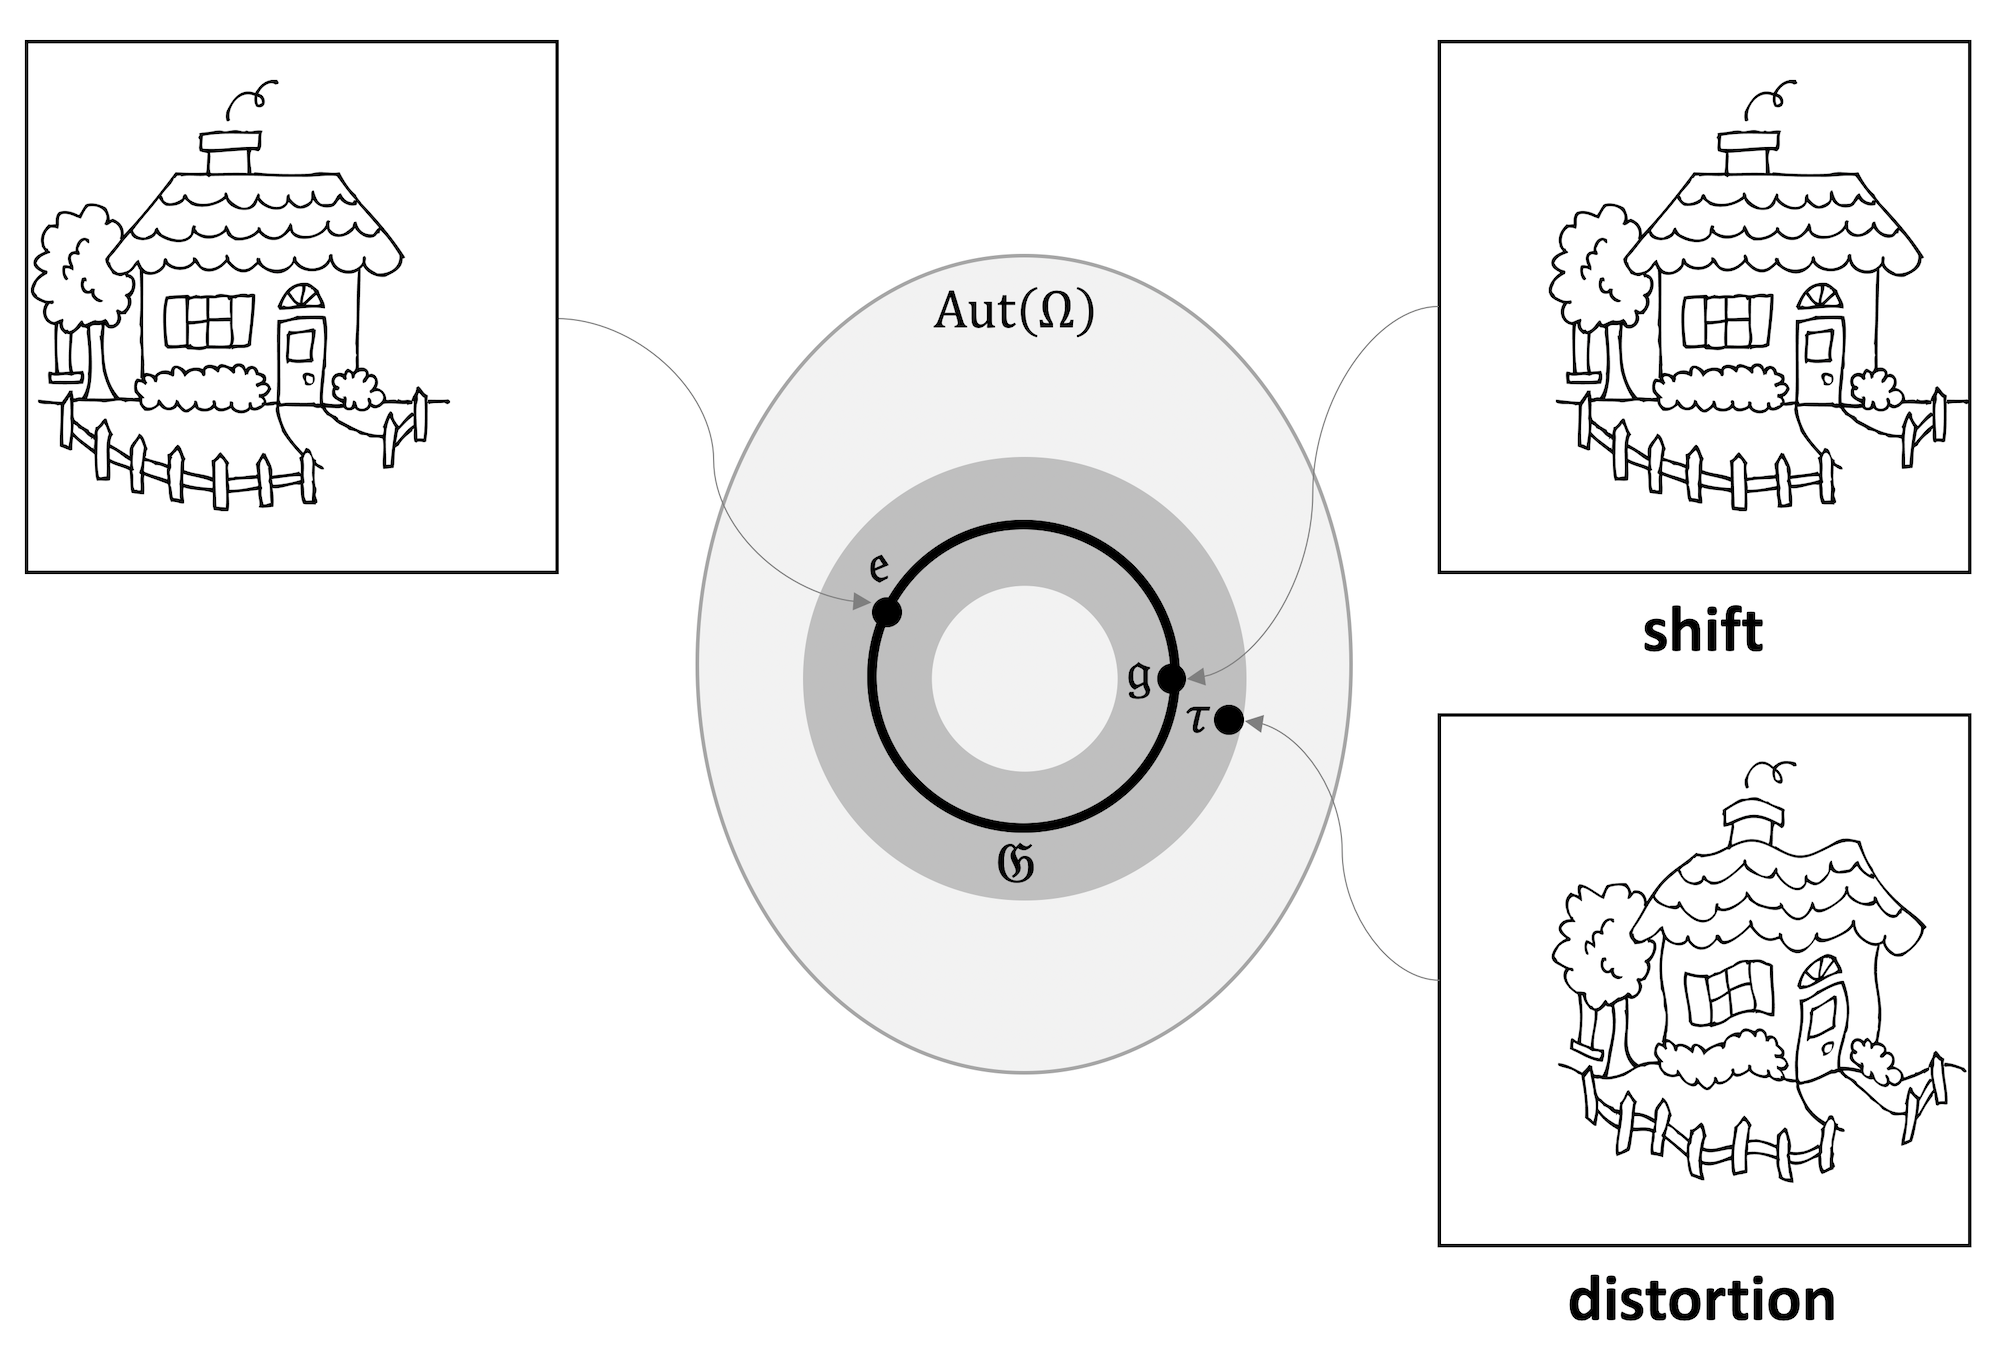
\includegraphics[width=1\textwidth]{figures/g_autg.png}
    \caption{The set of all bijective mappings from $\Omega$ into itself forms the \emph{set automorphism group}  $\mathrm{Aut}(\Omega)$, of which a symmetry group $\fG$ (shown as a circle) is a subgroup. Geometric Stability extends the notion of $\fG$-invariance and equivariance to `transformations around $\fG$' (shown as gray ring), quantified in the sense of some metric between transformations.
    In this example, a smooth distortion of the image is close to a shift. 
    }
    \label{fig:groupdeformation}
\end{figure}

%\begin{figure}
%    \centering
%    \includegraphics[width=0.7\textwidth]{figures/deform_image.pdf} \\
%    \includegraphics[width=0.7\textwidth]{figures/shapedef.pdf} \\
%        \includegraphics[width=0.4\textwidth]{figures/protein.jpg}
%    \caption{Examples of Deformations across different domains with a strong 
%    geometric stability prior. \michael{Better show a small molecule with a rotamer? Perhaps show just two examples of each?} }
%    \label{fig:deformation}
%\end{figure}

\paragraph{Stability to domain deformations}
In many applications, the object being deformed is not the signal, but the geometric domain $\Omega$ itself. Canonical instances of this are applications dealing with graphs and manifolds: a graph can model a social network at different instance of time containing slightly different social relations (follow graph), or a manifold can model a 3D object undergoing non-rigid deformations. 
%The intuition that one can slightly bend or twist a manifold can be formalized by considering a 
This deformation can be quantified as follows. If $\mathcal{D}$ denotes the space of all possible variable domains (such as the space of all graphs, or the space of Riemannian manifolds), one can define for $\Omega, \tilde{\Omega} \in \mathcal{D}$   an appropriate metric (`distance') $d(\Omega, \tilde{\Omega})$ satisfying $d(\Omega,\tilde{\Omega})=0$ if $\Omega$ and $\tilde{\Omega}$ are equivalent in some sense: for example, the graph edit distance vanishes when the graphs are isomorphic, and the Gromov-Hausdorff distance between Riemannian manifolds equipped with geodesic distances vanishes when two manifolds are isometric.\marginnote{The graph edit distance measures the minimal cost of making two graphs isomorphic by a sequences of graph edit operations. The Gromov-Hausdorff distance measures the smallest possible metric distortion of a correspondence between two metric spaces, see \cite{gromov1981structures}. } 


A common construction of such distances between domains relies on some family of 
%We assume that this metric comes with an 
invertible mapping $\eta: \Omega \to \tilde{\Omega}$ that try to `align' the domains in a way that the corresponding structures are best preserved. %This can be quantified for, %that is,
For example, in the case of graphs or Riemannian manifolds (regarded as metric spaces with the geodesic distance), this alignment can compare pair-wise adjacency or distance structures ($d$ and $\tilde{d}$, respectively),  %the alignment of graphs
%two graphs with $n$ nodes can be aligned 
%
$$d_{\gD}(\Omega, \tilde{\Omega}) =  \inf_{\eta \in \fG}\|d - \tilde{d}\circ (\eta \times \eta)\|$$
%
%$$d(\Omega, \Omega') = \inf_{\eta \in \fG} %\| e(\Omega) - \eta e(\Omega') \|~,$$
where $\fG$ is the group of isomorphisms such as bijections or isometries, and the norm is defined over the product space $\Omega \times \Omega$. In other words, a distance between elements of $\Omega,\tilde{\Omega}$ is `lifted' to a distance between the domains themselves, by accounting for all the possible alignments that preserve the internal structure.   
%rigid 
%symmetries of the domain 
%(e.g. permutations for graphs, or isometries for Riemannian manifolds), and $e(\cdot)$ is an embedding of the domain (such as the adjacency matrix for a graph, or an Euclidean embedding for a manifold). 
%\michael{Joan: please check. The assumptions on $\eta$ e.g. in GH-metric are very weak, just a bijection}
\marginnote{Two graphs can be aligned by the Quadratic Assignment Problem (QAP), which considers in its simplest form two graphs $G,\tilde{G}$ of the same size $n$, and solves $\min_{\mathbf{P} \in \Sigma_n} \mathrm{trace}(\mathbf{A P \tilde{A} P}^\top)$, where $\mathbf{A}, \tilde{\mathbf{A}}$ are the respective adjacency matrices and $\Sigma_n$ is the group of $n \times n$ permutation matrices. The graph edit distance can be associated with such QAP \citep{bougleux2015quadratic}.
}
Given a signal $x \in \gX(\Omega)$ and a deformed domain $\tilde{\Omega}$, one can then consider the deformed signal $\tilde{x} = x \circ \eta^{-1} \in \gX(\tilde{\Omega})$. 
%, $x' := x \circ \varphi^{-1}$.  
%For example, we can define a metri

%metric \emph{in the space of domains}. In other words, two graphs %$G, G'$ can be assigned a distance $d(G,G')$ so that $d(G,G')=0$ iff $G$ and $G'$ are isomorphic, and similarly two Riemannian manifolds $\Omega, \Omega'$ can be compared so that $d(\Omega, \Omega')$ measures the changes in their intrinsic metric structure. 

By slightly abusing the notation, we define $\gX(\mathcal{D}) = \{ (\gX(\Omega), \Omega) \, : \, \Omega \in \mathcal{D} \}$ as the ensemble of possible input signals defined over a varying domain. 
A function $f : \gX(\mathcal{D}) \to \gY$ is stable to domain deformations if 
\begin{equation}
\| f( x, \Omega) - f(\tilde{x}, \tilde{\Omega}) \| \leq C \|x \| d_{\gD}(\Omega, \tilde{\Omega})~
\label{eqn:domain_def_stability}
\end{equation}
%
for all $\Omega, \tilde{\Omega} \in \mathcal{D}$, and  $x \in \mathcal{X}(\Omega)$. 
%
%\michael{This is not properly defined: we have $x$ defined on both $\Omega$ and $\Omega'$, which requires some notion of correspondence} \joan{added some clarifications}. 
We will discuss this notion of stability in the context of manifolds in Sections~\ref{sec:manifolds}--\ref{sec:meshes}, where isometric deformations play a crucial role.
%As we will see in Chapter ??, 
Furthermore, it can be shown that the stability to domain deformations is a natural generalisation of the stability to signal deformations, by viewing the latter in terms of deformations of the volume form \cite{gama2019diffusion}. 

% %Link between the two via a change of variables. 
% In fact, the two notions of deformation stability are intimately related. Indeed, the deformation operator $L_\tau : \gX \to \gX$ acting on signals can be recast as deforming the inner-product metric, from $\gX = L^2(\Omega, du)$ to $L^2(\Omega,du_\tau)$. In other words, 
% $$\langle L_\tau x, L_\tau y \rangle_{L^2(\Omega), du)} = \int_\Omega x(\tau^{-1}(u)) y(\tau^{-1}(u)) du = \int_\Omega x(u) y(u) |\mathbf{I} - \nabla \tau^{-1}(u) | du := \int_\Omega x(u) y(u) du_\tau~,$$
% so we may view certain signal deformations as specific perturbations of the metric. 

%\michael{Measure not metric? or volume form? I find this section more confusing than helpful, we need to introduce a lot of extra stuff to make it defined properly} \joan{yes, agreed, i simply put a pointer for the future chapter to simplify things for now}. 



\subsection{Scale Separation}
\label{sec:scale_separation}

While deformation stability substantially strengthens the global symmetry priors, it is not sufficient in itself to overcome the curse of dimensionality, in the sense that, informally speaking, there are still ``too many" functions that respect (\ref{eq:defstability1}) as the size of the domain grows. A key insight to overcome this curse is to exploit the multiscale structure of physical tasks. Before describing multiscale representations, we need to introduce the main elements of Fourier transforms, which rely on frequency rather than scale. 

\paragraph{Fourier Transform and Global invariants}
Arguably 
\marginnote{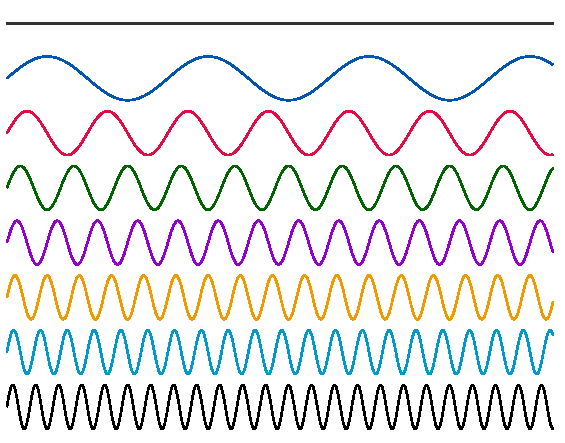
\includegraphics[width=\linewidth]{figures/fourier_basis.pdf}
Fourier basis functions have global support. As a result, local signals produce energy across all frequencies. 
}
the most famous signal decomposition is the {\em Fourier transform}, the cornerstone of harmonic analysis. 
%
The classical one-dimensional Fourier transform  
$$
\hat{x}(\xi) = \int_{-\infty}^{+\infty} x(u) e^{-\mi \xi u} \mathrm{d}u
$$
expresses the function $x(u) \in L^2(\Omega)$ on the domain $\Omega = \mathbb{R}$ as a linear combination 
of orthogonal oscillating {\em basis functions} $\varphi_\xi(u) = e^{\mi\xi u}$, 
indexed 
by their rate of oscillation (or \emph{frequency}) $\xi$. Such an organisation into frequencies reveals important information about the signal, e.g. its smoothness and localisation. 
%
%As we will show in Chapter ??, 
The Fourier basis itself has a deep geometric foundation and can be interpreted as the natural vibrations of the domain, related to its geometric structure (see e.g. \cite{berger2012panoramic}). 
%\marginnote{Technically, the Fourier transform is defined for functions in $L^2(\Omega) \cup L^1(\Omega)$, and can be extended to a far broader class of generalised functions through the theory of {\em tempered distributions} developed by the Fields laureate Laurent Schwartz. 
%We refer to \cite{mckean} for a wonderful treatment of Fourier Analysis

%

%\begin{figure}
%    \centering
%\includegraphics[width=0.5\linewidth]{figures/fourier1.pdf}
%    \caption{Basic decomposition of a signal into Fourier atoms. Observe that a localized discontinuity in the original signal produces energy across all frequencies.}
%    \label{fig:fourier}
%\end{figure}


%

% \joan{Michael, let me know if you agree. The following paragraph is not strictly needed in this section, and rather belongs to the grid/euclidean domain where we go again through this. I suggest we merge in there.} 
The Fourier transform\marginnote{In the following, we will use convolution and {\em (cross-)correlation} 
$$
(x \, \star \,\theta)(u) = \int_{-\infty}^{+\infty} \hspace{-2mm} x(v)\theta(u+v) \mathrm{d}v
$$
interchangeably, as it is common in machine learning: the difference between the two is whether the filter is reflected, and since the filter is typically learnable, the distinction is purely notational.
} plays a crucial role in signal processing as it offers a dual formulation of {\em convolution}, 
$$
(x\star \theta)(u) = \int_{-\infty}^{+\infty} x(v)\theta(u-v) \mathrm{d}v
$$
a standard model of linear signal filtering (here and in the following, $x$ denotes the signal and $\theta$ the filter). 
%
As we will show in the following, the convolution operator is diagonalised in the Fourier basis, making it possible to express convolution as the product of the respective Fourier transforms, 
$$
\widehat{(x\star \theta)}(\xi) = \hat{x}(\xi) \cdot \hat{\theta}(\xi),
$$
a fact known in signal processing as the Convolution Theorem. 
%
%In machine learning, convolution is the cornerstone of Convolutional Neural Networks, an architecture ubiquitously used in computer vision and image analysis applications. 


%Some of the properties of the Fourier transform are intimately related to the geometric properties of the Euclidean space or a grid on which it is defined.    
%The Fourier basis thus diagonalises any convolutional operator. 
As it turns out, many fundamental differential operators such as the Laplacian are described as convolutions on Euclidean domains. 
%, such as the Laplacian $\Delta = \mathrm{div} \, \nabla$. 
Since such differential operators can be defined intrinsically  over very general geometries, this provides a formal procedure to extend Fourier transforms beyond Euclidean domains, including graphs, groups and manifolds. We will discuss this in detail in Section~\ref{sec:manifolds}. %Chapter~???.

An essential aspect of Fourier transforms is that they reveal \emph{global} properties of the signal and the domain, such as smoothness or conductance. Such global behavior is convenient in presence of global symmetries of the domain such as translation, but not to study more general diffeomorphisms. This requires a representation that trades off spatial and frequential localisation, as we see next. 


\paragraph{Multiscale representations}
The 
%\marginnote{
%\includegraphics[width=0.9\linewidth]{figures/wavelet.pdf}
%Basic decomposition of a signal into wavelet atoms. Observe that now a localized discontinuity in the original signal creates energy only in the neighborhood of the discontinuity. 
notion of local invariance can be articulated by switching from a Fourier frequency-based representation to a {\em scale-based} representation, the cornerstone of multi-scale decomposition methods such as {\em wavelets}.\marginnote{See \cite{mallat1999wavelet} for a comperehensive introduction. } 
%; see Figure \ref{fig:fourier_vs_wavelets} and Insert ??. 
%
The essential insight of multi-scale methods is to decompose functions defined over the domain $\Omega$ into elementary functions that are localised \emph{both in space and frequency}.\marginnote{
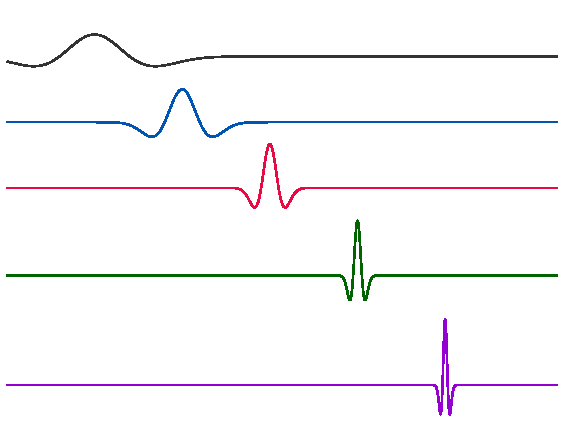
\includegraphics[width=0.9\linewidth]{figures/wavelet_basis.pdf}
%\includegraphics[width=0.9\linewidth]{figures/wavelet.pdf}
Contrary to Fourier, wavelet atoms are localised and multi-scale, allowing to capture 
fine details of the signal with atoms having small spatial
support and coarse details with atoms having large
spatial support.  
%Localized signals create energy only in the neighborhood of the discontinuity. 
The term \emph{ atom} here is synonymous with `basis element' in Fourier analysis, with the caveat that wavelets are redundant (over-complete).
}
In the case of wavelets, this is achieved by correlating a translated and dilated filter ({\em mother wavelet}) $\psi$, producing a combined spatio-frequency representation called a  {\em continuous wavelet transform} 
%
$$
(W_\psi x)(u,\xi) = \xi^{-1/2} \int_{-\infty}^{+\infty} 
\psi\left(\frac{v-u}{\xi}\right) x(v) \mathrm{d}v.
%psi( 2^{j} (u - k2^{-j})) 
%x(u) du \marginnote{In general, $\psi$ can be a complex-valued function, in which case a complex conjugation must be taken in the inner product.}
%(x \star \psi_j)(u)
$$
%
The translated and dilated filters are called {\em wavelet atoms}; % \marginnote{The term \emph{ atom} here is synonymous with `basis element' in Fourier analysis, with the caveat that wavelets are redundant representations that form over-complete bases.}
their spatial position and dilation correspond to the coordinates $u$ and $\xi$ of the wavelet transform. 
%
These coordinates are usually sampled dyadically ($\xi=2^{-j}$ and $u = 2^{-j}k$), with $j$ referred to as {\em scale}.  
%
%
%\int_{-\infty}^{+\infty} 
%\psi( 2^{j} (u - k2^{-j})) 
%x(u) du \marginnote{In general, $\psi$ can be a complex-valued function, in which case a complex conjugation must be taken in the inner product.}
%(x \star \psi_j)(u)
%$$
%
Multi-scale signal representations bring important benefits in terms of capturing regularity properties beyond global smoothness, such as piece-wise smoothness, which made them a popular tool in signal and image processing and numerical analysis in the 90s. 

\paragraph{Deformation stability of Multiscale representations:}
The benefit of multiscale localised wavelet decompositions over Fourier decompositions is revealed when considering the effect of small deformations `nearby' the underlying symmetry group. Let us illustrate this important concept in the Euclidean domain and the translation group.   
Since the Fourier representation diagonalises the shift operator (which can be thought of as convolution, as we will see in more detail in  Section~\ref{sec:grids_euclidean}), it is an efficient representation for translation transformations. However, Fourier decompositions are unstable under high-frequency deformations. 
%
In contrast, wavelet decompositions offer a stable representation in such cases. 

Indeed, let us consider $\tau \in \mathrm{Aut}(\Omega)$ and its associated linear representation $\rho(\tau)$. When $\tau(u) = u - v$ is a shift, 
as we will verify in Section \ref{sec:grids_euclidean}, the operator $\rho(\tau) = S_v$ is a {\em shift operator} that commutes with convolution. 
%any convolution operator $H$ of the form $H x = x \star h$, with arbitrary filter $h$. 
Since convolution operators are diagonalised by the Fourier transform, the action of shift in the frequency domain amounts to shifting the complex phase of the Fourier transform,  
%
%As a result, by expressing this commutation relationship in the Fourier domain, we have that 
$$
(\widehat{S_v x})(\xi) = e^{-\mi \xi v} \hat{x}(\xi). 
$$ 
%for any frequency $\xi$. 
%Rigid translations are thus expressed in the Fourier domain by simply shifting the (complex) phase of every fourier coefficient of the signal, leading 
Thus, the {\em Fourier modulus} $f(x) = |\hat{x}|$ removing the complex phase is a simple shift-invariant function, $f(S_v x) = f(x)$. 
%to simple translation invariant representations by removing this complex phase: $Mx = |\hat{x}|$. In other words, for rigid translations, the Fourier modulus is translation invariant: $\| M - M L_\tau \| = 0$. 
%
However, if we have only approximate translation, 
%$\tau(u) \approx u - v$, 
$\tau(u) = u - \tilde{\tau}(u)$ with $\|\nabla \tau \|_\infty = \sup_{u\in \Omega} \| \nabla \tilde{\tau}(u)\| \leq \epsilon$,  
the situation is entirely different: it is possible to show that 
$$
\frac{\|f(\rho(\tau) x) - f(x) \| }{ \|x\| }= \mathcal{O}(1)
$$ 
irrespective of how small $\epsilon$ is (i.e., how close is $\tau$ to being a shift). Consequently, such Fourier representation is {\em unstable under deformations}, however small. This unstability is manifested in general domains and non-rigid transformations; we will see another instance of this unstability in the analysis of 3d shapes using the natural extension of Fourier transforms described in Section \ref{sec:geomanifoldsec}. 

Wavelets offer a remedy to this problem that also reveals the power of multi-scale representations. In the above example, we can show \citep{mallat2012group} that the wavelet decomposition $W_\psi x$ is {\em approximately equivariant} to deformations,
$$
\frac{\| \rho(\tau) (W_\psi x) - W_\psi (\rho(\tau) x) \|}{\|x\|} = \mathcal{O}(\epsilon).
\marginnote{This notation implies that $\rho(\tau)$ acts on the spatial coordinate of $(W_\psi x)(u,\xi)$.
}
$$
%and $\gW x = \{ x \star \psi_j \}_j$ is an appropriately normalized wavelet filter bank, then one can verify that wavelet coefficients are nearly \emph{equivariant} to deformations, in the sense that $\| L_\tau \gW - \gW L_\tau \| = O(\epsilon)$. 
%
In other words, decomposing the signal information into scales using localised filters rather than frequencies turns a global unstable representation into a family of locally stable features. Importantly, such measurements at different scales are not yet invariant, and need to be progressively processed towards the low frequencies, hinting at the deep compositional nature of modern neural networks, and captured in our Blueprint for Geometric Deep Learning, presented next. 


% From our discussion 
% Let us consider a filter $h(u)$ and its associated convolution operator $\gH x = x \star h$. To study how this operator behaves under certain geometric transformations $L_\tau \in \mathrm{Aut}(\Omega)$ we consider the \emph{Lie commutator} 

% Let us consider the Lie commutator $[L_\tau, \gW]= L_\tau \gW - \gW L_\tau$. When $\gW$ is the Fourier transform and $L_\tau$ is exactly a translation, we have $[L_\tau, \gW] = 0$; 
% %Let us denote the decomposition by $U$ and let $L_\tau$ be the deformation operator we have seen before. When $\tau(u) = u-v$ is a pure translation, the Fourier transform satisfies $L_\tau U = U L_\tau$, by virtue of its 
% however when $L_\tau$ is only an approximate translation, then $\| [L_\tau, \gW] \| = O(1)$, irrespective of how close $L_\tau$ is to being a translation. 
% On the other hand, if $\tau(u) = u - \tilde{\tau}(u)$, with $\sup_u \| \nabla \tilde{\tau}(u)\| \leq \epsilon$ (thus $\tau$ is nearly a translation), then one can show \cite{scatt} that when $\gW$ is the overcomplete wavelet transform, $\| [ L_\tau, \gW ] \| \simeq \epsilon$. 





%\paragraph{Scale Separation}
%In our context of high-dimensional learning, multiscale representations such as wavelets serve another fundamental purpose: they provide overcomplete linear decompositions where local translations are nearly equivariant.  
\paragraph{Scale Separation Prior: }
We can build from this insight by considering a multiscale coarsening of the data domain $\Omega$ into a hierarchy $\Omega_1, \hdots, \Omega_J$. 
%, $j\in [J]$. 
As it turns out, such coarsening can be defined on very general domains, including grids, graphs, and manifolds. 
%capturing a wide range of applications.
Informally, a coarsening assimilates nearby points $u, u' \in \Omega$ together, and thus only requires an appropriate notion of {\em metric} in the domain. 
%Geometric objects such as grids, manifolds, Lie groups or Graphs all admit such coarsenings. 
If $\gX_{j}(\Omega_j,\mathcal{C}_j) := \{x_j: \Omega_j \to \mathcal{C}_j \}$ 
%\michael{\bf [MB: why $\R^s$? did not we assume scalar-valued signals for simplicity? ]} 
%\joan{JB: number of channels can vary as we coarsen the domain. But we should keep things simple at this stage, and just describe the general principle without introducing too much notation. } \michael{MB: lets keep it as simple as possible here} 
denotes signals defined over the coarsened domain $\Omega_j$, we informally say that a function $f : \gX(\Omega) \to \gY$ is \emph{locally stable} at scale $j$ if it admits a factorisation of the form $f \approx f_j \circ P_j $, where $P_j : \gX(\Omega) \to \gX_{j}(\Omega_j)$ is a non-linear \emph{coarse graining} and $f_j : \gX_{j}(\Omega_j) \to \gY$. In other words, while the target function $f$ might depend on complex long-range interactions between features over the whole domain, in locally-stable functions it is possible to \emph{separate} the interactions across scales, by first focusing on localised interactions that are then propagated towards the coarse scales. 

\begin{figure}
    \centering
    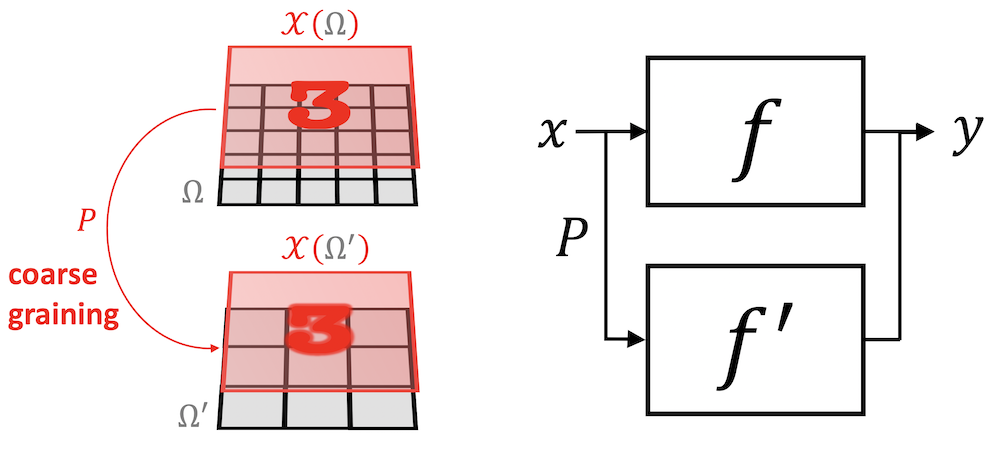
\includegraphics[width=0.75\textwidth]{figures/scale_sep.png}%factorization.pdf}
    \caption{Illustration of Scale Separation for image classification tasks. The classifier $f'$ defined on signals on the coarse grid $\mathcal{X}(\Omega')$ should satisfy $f \approx f'\circ P$, where $P: \mathcal{X}(\Omega) \rightarrow \mathcal{X}(\Omega')$. }
    \label{fig:scale_separation}
\end{figure}

Such principles\marginnote{Fast Multipole Method (FMM) is a numerical technique originally developed to speed up the calculation of long-ranged forces in $n$-body problems. FMM groups sources that lie close together and treats them as a single source.
} are of fundamental importance in many areas of physics and mathematics, as manifested for instance in statistical physics in the so-called renormalisation group, or leveraged in important numerical algorithms such as the Fast Multipole Method. In machine learning, multiscale representations and local invariance are the fundamental mathematical principles underpinning the efficiency of Convolutional Neural Networks and Graph Neural Networks and are typically implemented in the form of {\em local pooling}. In future work, we will further develop tools from computational harmonic analysis that unify these principles across our geometric domains and will shed light onto the statistical learning benefits of scale separation. 





\subsection{The Blueprint of Geometric Deep Learning}
\label{sec:gdl_blueprint}

The geometric principles of Symmetry, Geometric Stability, and Scale Separation discussed in Sections~\ref{sec:symmetries}--\ref{sec:scale_separation} can be combined to provide a universal blueprint for learning stable representations of high-dimensional data. 
%
These representations will be produced by functions $f$ operating on signals $\mathcal{X}(\Omega,\mathcal{C})$ defined on the domain $\Omega$, which is endowed with a symmetry group $\fG$. 


The geometric priors we have described so far do not prescribe a specific {\em architecture} for building such representation, but rather a series of necessary conditions. 
However, they hint at an axiomatic construction that provably satisfies these geometric priors, while ensuring a highly expressive representation that can approximate any target function satisfying such priors. %the geometric priors. 


A simple initial observation is that, in order to obtain a highly expressive representation, we are required to introduce a non-linear element, since
if $f$ is linear and $\fG$-invariant, then for all $x \in \gX(\Omega)$, \marginnote{Here, $\mu(\fg)$ is known as the \emph{Haar measure} of the group $\fG$, and the integral is performed over the entire group.}
$$
f(x) =  \frac{1}{\mu(\fG)} \int_{\fG} f( \fg. x) \mathrm{d}\mu(\fg) = f\left(\frac{1}{\mu(\fG)} \int_{\fG} (\fg.x) \mathrm{d}\mu(\fg) \right),
$$
%\michael{f(x) and not F?}
%\michael{what is $\fg.x$? should be u or use representation $\rho$}
which indicates that $F$ only depends on $x$ through the  \emph{$\fG$-average} $A{x} = \frac{1}{\mu(\fG)} \int_{\fG} (\fg.x) \mathrm{d}\mu(\fg)$. In the case of images and translation, this would entail using only the average RGB color of the input! %\marginnote{Give a further example for the discrete permutation group, getting the average too}


While this reasoning shows that the family of {\em linear invariants} is not a very rich object, the family of {\em linear equivariants} provides a much more powerful tool, since it enables the construction of rich and stable features by composition with appropriate non-linear maps, as we will now explain. 
%
Indeed, if $B: \gX(\Omega, \gC) \to \gX( \Omega, \gC')$ is $\fG$-equivariant satisfying $B(\fg.x) = \fg.B(x)$ for all $x \in \gX$ and $\fg \in \fG$, and $\sigma: \gC' \to \gC''$ is an arbitrary (non-linear) map, then we easily verify that the composition $U := (\bm{\sigma} \circ B): \gX(\Omega, \gC) \to \gX( \Omega, \gC'')$ is also $\fG$-equivariant, where $\bm{\sigma}: \gX(\Omega,\gC') \to \gX(\Omega, \gC'')$ is the element-wise instantiation of $\sigma$ given as $(\bm{\sigma}(x))(u) := \sigma( x(u))$.

This simple property allows us to define a very general family of $\fG$-invariants, by composing $U$ with the group averages $A \circ U : \gX(\Omega, \gC) \to \gC''$. A natural question is thus whether any $\fG$-invariant function can be approximated at arbitrary precision by such a model, for appropriate choices of $B$ and $\sigma$. 
%
It is not hard to adapt the standard Universal Approximation Theorems from unstructured vector inputs to show that shallow `geometric' networks are also universal approximators, by properly generalising the group average to a general non-linear invariant. 
\marginnote{Such proofs have been demonstrated, for example, for the Deep Sets model by \citet{zaheer2017deep}.}
%
However, as already described in the case of Fourier versus Wavelet invariants, there is a 
fundamental tension between shallow global invariance and deformation stability.
This motivates an alternative representation, which considers instead \emph{localised} equivariant maps.\marginnote{Meaningful metrics can be defined on grids, graphs, manifolds, and groups. A notable exception are sets, where there is no predefined notion of metric. 
%; see Section ? for further discussion.
} 
Assuming that $\Omega$ is further equipped with a distance metric $d$, we call an equivariant map $U$ localised if $(Ux)(u)$ depends only on the values of $x(v)$ for $\mathcal{N}_u = \{v : d(u,v) \leq r\}$, for some small radius $r$; the latter set $\mathcal{N}_u$ is called the {\em receptive field}. %$\delta$; . 
%\michael{Are we ok to indentify neighbourhood with receptive field?}

A single layer of local equivariant map $U$ cannot approximate functions with long-range interactions, but a composition of several local equivariant maps $U_J \circ U_{J-1} \dots \circ U_1$ increases the receptive field\marginnote{The term `receptive field' originated in the  neuroscience literature, referring to the spatial domain that affects the output of a given neuron.}  while preserving the stability properties of local equivariants. The receptive field is further increased by interleaving downsampling operators that coarsen the domain (again assuming a metric structure), completing the parallel with Multiresolution Analysis (MRA, see e.g. \cite{mallat1999wavelet}). 

\begin{figure}
    \centering
    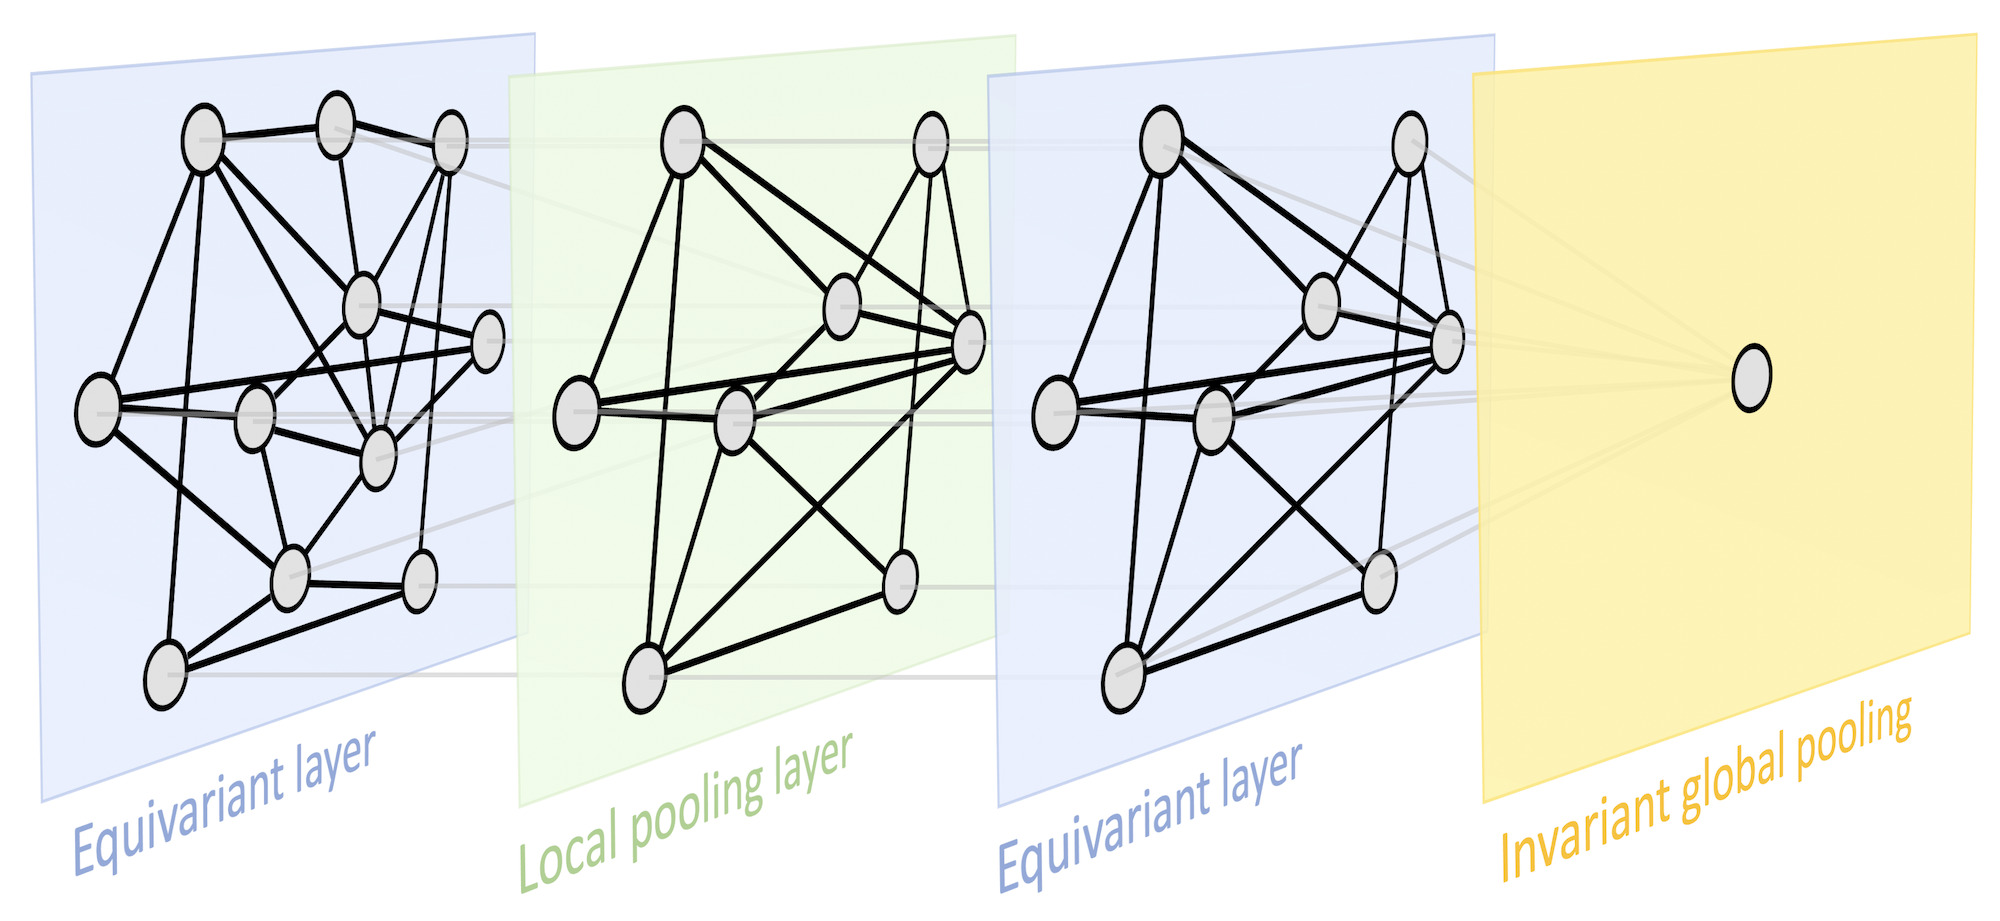
\includegraphics[width=1\textwidth]{figures/blueprint.png}
    \caption{Geometric Deep Learning blueprint, exemplified on a graph. A typical Graph Neural Network architecture may contain permutation equivariant layers (computing node-wise features), local pooling (graph coarsening), and a permutation-invariant global pooling layer (readout layer). }
    \label{fig:blueprint}
\end{figure}

In summary, the geometry of the input domain, with knowledge of an underyling symmetry group, provides three key building blocks: (i) a local equivariant map, (ii) a global invariant map, and (iii) a coarsening operator. These building blocks provide a rich function approximation space with prescribed invariance and stability properties by combining them together in a scheme we refer to as the  
%
\emph{Geometric Deep Learning Blueprint} (Figure~\ref{fig:blueprint}). 
%
%We will see that a large number of popular neural network architectures used in deep representation learning are particular instances of this blueprint, illustrated in 
%across all the geometric domains we will describe next. 
%



%\begin{tcolorbox}[width=\linewidth,
%                  boxsep=0pt,
%                  left=7.5pt,
%                  right=7.5pt,
%                  top=7.5pt,
%                  bottom=7.5pt,
%                  arc=0pt,
%                  boxrule=0pt,toprule=0pt,
%                  colback=boxgray,
%                  ]%%
    
%\begin{center}
%Given a hierarchy of domains $\Omega_J \subseteq \hdots \subseteq \Omega_2 \subseteq \Omega_1 = \Omega$ with symmetry group $\fG$, the 
%\textbf{Geometric Deep Learning Blueprint} allows constructing $\fG$-invariant functions $f:\mathcal{X}(\Omega,\mathcal{C}) \rightarrow \mathcal{Y}$ of the form 
%$$
%f = A \circ \boldsymbol{\sigma}_J \circ U_J \circ P_{J-1} \circ \hdots \circ P_1 \circ \boldsymbol{\sigma}_1 \circ B_1
%$$
%consisting  of the following building blocks:\\

%    \noindent {\em Linear $\fG$-equivariant layer} $B_j: \gX(\Omega_j, \gC_j) \to \gX( \Omega_{j}, \gC'_{j})$ satisfying $B(\fg.x) = \fg.B(x)$ for all $\fg \in \fG$ and $x\in \gX(\Omega_j,\mathcal{C}_j)$. 
%    \vspace{2mm}\\

%    \noindent {\em Nonlinearity} $\sigma_j: \gC'_j \to \gC_j$ applied element-wise as $(\bm{\sigma}(x))(u) = \sigma( x(u))$.\vspace{2mm}\\\

%    \noindent {\em Local pooling (coarsening)}  $P_j : \gX(\Omega_j, \gC_j) \rightarrow \gX(\Omega_{j+1}, \gC_{j+1}) $.\vspace{2mm}\\
    
%    \noindent {\em Invariant layer (global pooling) } $A: \gX(\Omega_J, \gC_J) \rightarrow \mathcal{Y}$ satisfying $A(\fg .x) = A(x)$ for all $\fg \in \fG$ and $x\in \gX(\Omega_J,\mathcal{C}_J)$.  %.\vspace{2mm}\\

%\end{center}
%\end{tcolorbox}


\begin{tcolorbox}[width=\linewidth,
                  boxsep=0pt,
                  left=7.5pt,
                  right=7.5pt,
                  top=7.5pt,
                  bottom=7.5pt,
                  arc=0pt,
                  boxrule=0pt,toprule=0pt,
                  colback=boxgray,
                  ]%%
    
\begin{center}
\textbf{Geometric Deep Learning Blueprint}
\end{center}
Let $\Omega$ and $\Omega'$ be domains, $\fG$ a symmetry group over $\Omega$, and write $\Omega' \subseteq \Omega$ if $\Omega'$ can be considered a compact version of $\Omega$. \\

We define the following building blocks:\vspace{2mm}\\

    \noindent {\em Linear $\fG$-equivariant layer} $B: \gX(\Omega, \gC) \to \gX( \Omega', \gC')$ satisfying $B(\fg.x) = \fg.B(x)$ for all $\fg \in \fG$ and $x\in \gX(\Omega,\mathcal{C})$.\vspace{2mm}\\

    \noindent {\em Nonlinearity} $\sigma: \gC \to \gC'$ applied element-wise as $(\bm{\sigma}(x))(u) = \sigma( x(u))$.\vspace{2mm}\\

    \noindent {\em Local pooling (coarsening)}  $P : \gX(\Omega, \gC) \rightarrow \gX(\Omega', \gC) $, such that $\Omega'\subseteq\Omega$.\vspace{2mm}\\
    
    \noindent {\em $\fG$-invariant layer (global pooling) } $A: \gX(\Omega, \gC) \rightarrow \mathcal{Y}$ satisfying $A(\fg .x) = A(x)$ for all $\fg \in \fG$ and $x\in \gX(\Omega,\mathcal{C})$.\vspace{2mm}\\

Using these blocks allows constructing $\fG$-invariant functions $f:\mathcal{X}(\Omega,\mathcal{C}) \rightarrow \mathcal{Y}$ of the form 
$$
f = A \circ \boldsymbol{\sigma}_J \circ B_J \circ P_{J-1} \circ \hdots \circ P_1 \circ \boldsymbol{\sigma}_1 \circ B_1
$$
where the blocks are selected such that the output space of each block matches the input space of the next one. Different blocks may exploit different choices of symmetry groups $\fG$.
\end{tcolorbox}

%


% A natural question is then how expressive this generic construction is in the class of $\fG$-invariant functions, and, equally important, which conditions on $B$ and $\rho$ ensure geometric stability.  
% Universal Approximation

% A simple option to ensure rich and stable representations is to instead compose several \emph{layers} of non-linear local equivariant maps before applying the global invariant. 

% The idea of deep learning is to define $f$ as a \emph{composition} of maps (or ``layers'').
% These maps should be compatible in that the output space of one layer should match the input space of the next layer.
% %That is, we can compose $f_1 : \mathcal{X}(\Omega, \mathcal{C}) \rightarrow \mathcal{X}(\Omega', \mathcal{C}')$ and $f_2 : \mathcal{X}(\Omega'', \mathcal{C}'') \rightarrow \mathcal{X}(\Omega''', \mathcal{C}''')$ if and only if $\mathcal{X}(\Omega', \mathcal{C}') = \mathcal{X}(\Omega'', \mathcal{C}'')$.
% That is, we can compose $f_1 : \mathcal{X}_1 \rightarrow \mathcal{X}_2$ and $f_2 : \mathcal{X}_2' \rightarrow \mathcal{X}_3$ if and only if $\mathcal{X}_2 = \mathcal{X}_2'$ (where we have abbreviated $\mathcal{X}_i = \mathcal{X}(\Omega_i, \mathcal{C}_i)$).
% Whereas in regular deep learning, maps can be composed as soon as the input and output spaces match as \emph{vector spaces} (i.e. they have the same dimensionality / array shape), in geometric deep learning these spaces should match as \emph{group representations}.
% This means that, in addition to matching as vector spaces, the group $\fG$ should act in the same way on both spaces.
% When this is the case, equivariance of $f_1$ and $f_2$ implies equivariance of the composition $f_2 \circ f_1$.

% Most networks in geometric deep learning are compositions of a few basic building blocks:

% %\emph{Local} 
% $\fG$-\emph{equivariant} linear operator $A: \gX(\Omega) \to \gX_{\gV'}(\Omega)$ satisfying $A(\fg.x) = \fg. A(x)$ for any $x \in \mathcal{X}(\Omega)$ and $\fg\in\fG$. 
% %
% Typically, this operator is further assumed to be {\em local}, i.e. $(Ax)(u)$ depends only on the values of $x(v)$ for $v$ in the vicinity of $u$, in the sense of some metric on $\Omega$.  
% %and such that $A x(u)$ only depends upon $\{ x(v); \mathrm{g}(v,u) \leq \delta\}$, where $\delta$ encodes the size of the neighborhood. 

% \emph{Pointwise nonlinearity} $\sigma: \mathcal{C}' \to \mathcal{C}''$. Under our assumptions, this implies that $\sigma \circ A$ is local and $\fG$-\emph{equivariant} whenever $A$ is such. \marginnote{When $\sigma$ acts coordinate-wise, it is typically referred to as an \emph{activation function}. In general,  $\sigma$ can be a generic function, such as a fully-connected neural network. }

% % \joan{
% % Argue that the only linear $\fG$-invariant is the group average. 
% % If $F$ is linear and $\fG$-invariant, then for all $x$, 
% % $$F(x) =  \frac{1}{\mu(\fG)} \int F( g.x) \mu(dg) = F\left(\frac{1}{\mu(\fG)} \int g.x \mu(dg) \right)~,$$
% % so $F$ only depends on $x$ through the average. 

% % This justifies why we need to add non-linearities
% % }




% {\em Local pooling} (or downsampling operator) $P_j: \gX(\Omega_j,\mathcal{C}_{j}) \to \gX(\Omega_{j+1},\mathcal{C}_{j+1})$ defined on a hierarchy of domains $\Omega_1, \hdots, \Omega_J$. 
% %reducing the resolution of the domain. 

% {\em Global pooling} $\fG$-{\em invariant} operator $a:\mathcal{X}(\Omega,\mathcal{C}) \rightarrow \mathcal{Y}$. 
    



% %
% %\michael{\bf [MB: INSERT FIGURE of a general equivariant/invariant architecture, similarly to Maron's thesis]}
% %
% %Let $\gX(\Omega, \gV) := \{ x : \Omega \to \gV \}$ be the input space, with domain $\Omega$ and feature space $\gV$ . We assume a metric $\mathrm{g}$ on $\Omega$ and a symmetry group $\fG$ acting on it, which also defines a linear representation 
% %%(taco confirm language? \taco{Correct. This is called the regular rep of G on X. Will add a definition to 1.2.1}) 
% %over $\gX$ by composition, as in Figure \ref{fig:symmetryactors}.
% %%if $x \in \gX$ and $g \in \fG$, then $g x (u) = x(gu) \in \R^s$. [we assume that the group does not act along channels for now]
% %\taco{TODO: add condition that signal space should have an inner product, i.e. be a Hilbert space. See definition box in 1.2}
% %
% %The GDL blueprint consists of four fundamental building blocks that are composed together appropriately:
% %\begin{enumerate}
% %    \item A \emph{local} $\fG$-\emph{equivariant} linear operator $A: \gX_{\gV}(\Omega) \to \gX_{\gV'}(\Omega)$; that is, $A(\fg.x) = \fg. A(x)$ for any $x$ and $\fg$, and such that $A x(u)$ only depends upon $\{ x(v); \mathrm{g}(v,u) \leq \delta\}$, where $\delta$ encodes the size of the neighborhood. 
% %    \item A \emph{nodewise} nonlinear activation function $\sigma: \gV' \to \gV''$. Under our assumptions, this implies that $\sigma \circ A$ is local and $\fG$-\emph{equivariant} whenever $A$ is as above. When $\text{dim}(\gV')=\text{dim}(\gV'')=1$, $\sigma$ is typically described as an \emph{activation function}, but in general $\sigma$ can be a generic function, such as a fully-connected neural network. 
% %    \item Local pooling or downsampling operator $P_k: \gX_{\gV}(\Omega_k) \to \gX_{\gV}(\Omega_{k+1})$ reducing the resolution of the domain. 
% %    \item Global pooling: $\fG$-invariant operator. 
% %\end{enumerate}




% %\michael{MB: I am in favor of keeping the blueprint as simple as possible even at the expense of precision of definitions/generality. It should be intuitive and I feel currently the intuition is buried under too much notation. }


% The majority of deep neural networks implement a composition of multiple such components of the form
% $$
% f =a \circ P_L \circ \sigma_L \circ A_L \dots P_1 \circ \sigma_1 \circ A_1,
% $$
% with each component referred to as a {\em layer}. The term `deep' is used to indicate that there are many such layers, though we should say that how deep is deep is in the eyes of the beholder.\marginnote{Some CNN architectures used in computer vision can have hundreds of layers. }
% %
% %The multilayer composition $f =a \circ P_L \circ \sigma_L \circ A_L \dots P_1 \circ \sigma_1 \circ A_1$ 
% %
% Such a multilayer construction allows to define a flexible functional space with prescribed geometric priors. On the one hand, the equivariant nature of the maps $\sigma \circ A_j$ is preserved under composition, resulting in overall invariance when composed with a global pooling operator. On the other hand, the use of pooling layers allows to exploit the scale separation prior. 

\paragraph{Different settings of Geometric Deep Learning}
One can make an important distinction between the setting when the domain $\Omega$ is assumed to be {\em fixed} and one is only interested in varying input signals defined on that domain, or the domain is part of the input as {\em varies} together with signals defined on it. 
%
A classical instance of the former case is encountered in computer vision applications, where images are assumed to be defined on a fixed domain (grid). 
%
Graph classification is an example of the latter setting, where both the structure of the graph as well as the signal defined on it (e.g. node features) are important. 
%
In the case of varying domain, geometric stability (in the sense of insensitivity to the deformation of $\Omega$) plays a crucial role in Geometric Deep Learning architectures. 


This blueprint  has the right level of generality to be used across a wide range of geometric domains. 
Different Geometric Deep Learning methods thus differ in their choice of the domain, symmetry group, and the specific implementation details of the aforementioned building blocks. 
%and the metric defining locality. 
As we will see in the following, a large class of deep learning architectures currently in use fall into this scheme and can thus be derived from common geometric principles.  
%
%We will now discuss specific instances of this blueprint and how it adapts to each case.  


In the following sections~(\ref{sec:proto-graphs}--\ref{sec:meshes}) we will describe the various geometric domains focusing on the `5G', and in Sections~\ref{sec:cnnsec}--\ref{sec:lstm} the  specific implementations of Geometric Deep Learning on these domains. 



%Such generic architecture, illustrated in Figure~\ref{fig:blueprint}, can be instantiated across a variety of domains with different geometric structures giving rise to a very large zoo of architectures united by these common geometric principles. Let us now discuss these domains and how this blueprint adapts to each case. 


% First, we define a collection of \emph{local} $\fG$-\emph{equivariant} linear operators. In  deep learning architectures such as CNNs and GNNs these correspond to convolutional and message passing layers, and the corresponding groups are translation and permutation, respectively. 

% Next, these operators are composed with a non-linearity called an {\em activation function} in the neural networks jargon, which preserves the equivariance as it is applied element-wise. \taco{TC: note that element-wise nonlinearities are only equivariant to certain kinds of group representations, namely when the representation matrices are all permutation matrices}

% Finally, coarsen the representations produced by the equivariant operators. In image analysis applications, this is achieved by means of {\em pooling}, an operation reducing the size of the image grid, and as we shall see next, coarsening may be defined on far more general data domains.

% In an idealised instantiation, the coarsening is performed at the output. It can be shown that this representation is 
% provably $\fG$-invariant/equivariant, and that the locality assumption captures the scale separation inductive bias. 
% Moreover, such representations are universal approximators under symmetry, as we discuss in Chapter ??. 

%\joan{Joan: Taco, we can generalise the blueprint to accommodate more group representations, if we feel the use cases are sufficiently important. Otherwise, an alternative is to mention that this blueprint can be extended in some domains to account for special types of group actions}

%\taco{Taco: Joan, I agree we really only need reps that describe how signals transform. However that is still a bit more general than $\rho(\fg) x(u) = x(\fg^{-1} u)$. In particular for steerable cnns / induced reps, as well as gauge cnns, we have some smaller group acting on the feature vector. E.g. a vector field on the sphere transforms according to the rep of SO3 that is induced by the vector rep of SO2 acting on 2D vectors. 

%One option is to ignore this for now and call this the ``deep learning blueprint (simplified)'', and mention that we need something slightly more general. We can introduce the full thing in a separate chapter. Only downside is that we cannot write the gauges section of the intro to conform to the simplified blueprint then. May not be such a big deal...

%Alternatively, we can first introduce a general definition for arbitrary reps, then introduce one specialized version for $\rho(\fg) x(u) = x(\fg^{-1} u)$. Then later we can say in the gauges section that the gauge story fits the general blueprint but involves a different kind of rep.
%}


%(either explicitly or implictly since energy is pushed towards low frequencies).
    

%\begin{enumerate}
%    \item Define a collection of \emph{local}, $\gG$-\emph{equivariant} linear operators $U_m$. 
%    \item Compose them with an element-wise non-linearity $\rho$. 
%    \item Coarsen the hidden representations (either explicitly or %implictly since energy is pushed towards low frequencies).
%\end{enumerate}





\begin{tcolorbox}[width=\linewidth,
                  boxsep=0pt,
                  left=7.5pt,
                  right=7.5pt,
                  top=7.5pt,
                  bottom=7.5pt,
                  arc=0pt,
                  boxrule=0pt,toprule=0pt,
                  colback=boxgray,
                  ]%%
    
\begin{center}
%\textbf{Geometric Deep Learning Blueprint}\newline
\begin{tabular}{lll}
     {\bf Architecture} & {\bf Domain} $\Omega$ & {\bf Symmetry group} $\mathfrak{G}$\vspace{2.5mm}\\
     {\em CNN} & Grid & Translation\vspace{2mm}\\
%
     {\em Spherical CNN} & Sphere / $\mathrm{SO}({3})$ & Rotation $\mathrm{SO}({3})$\vspace{2mm}\\

     {\em Intrinsic / Mesh CNN} & Manifold & Isometry $\mathrm{Iso}(\Omega)$ / \\
     & & Gauge symmetry $\mathrm{SO}(2)$\vspace{2mm}\\     


     {\em GNN} & Graph & Permutation  $\Sigma_n$\vspace{2mm}\\     

     {\em Deep Sets} & Set & Permutation $\Sigma_n$\vspace{2mm}\\     
     {\em Transformer} & Complete Graph & Permutation $\Sigma_n$\vspace{2mm}\\
     {\em LSTM} & 1D Grid & Time warping\\     


\end{tabular}
\end{center}
\end{tcolorbox}
%

%\begin{tcolorbox}[width=\linewidth,
%                  boxsep=0pt,
%                  left=7.5pt,
%                  right=7.5pt,
%                  top=7.5pt,
%                  bottom=7.5pt,
%                  arc=0pt,
%                  boxrule=0pt,toprule=0pt,
%                  colback=boxgray,
%                  ]%%
%    
%\begin{center}
%\textbf{Geometric Deep Learning Blueprint instances of interest}\newline
%\begin{tabular}{cccc}
%     Domain, $\Omega$ & Metric, $g$ & Symmetry group, $\frak{G}$ & Architecture\\
%     {\bf Grids} & $L_\infty$ & Translations & {\bf CNNs}\\ 
%     {\bf Spheres} & Great circle & \multirow{2}{*}{3D rotations, SO(3)} & \multirow{2}{*}{\bf Spherical CNNs} \\
%     {\bf SO(3)} & Geodesic & \\
%     \multirow{2}{*}{\bf Gauges} & \multirow{2}{*}{Geodesic} & \multirow{2}{*}{\{Gauge transform.\}} & {\bf Gauge Equivariant} \\ & & & {\bf Mesh CNNs} \\
%     {\bf Graphs} & Shortest path & Permutations, $\Sigma_n$ & {\bf GNNs}\\
%     \multirow{2}{*}{\bf Sets} & $+\infty$ & Permutations, $\Sigma_n$ & {\bf Deep Sets}\\
%     & $0$ & Permutations, $\Sigma_n$ & {\bf Transformers}\\
%\end{tabular}
%\end{center}
%\end{tcolorbox}


%\begin{figure}
%    \centering
%    \includegraphics[width=0.9\textwidth]{figures/equivariant-network-blueprint.png}
%    \caption{todo}
%    \label{fig:equivariant-net-blueprint}
%\end{figure}




%\michael{\bf [MB: give examples here?]}



%{\bf 
%Main questions:

%What the equivariant structure that is required at every hidden %layer. 
%Universality vs efficiency. 

%Generalization?
%}

%Scale separation in neural networks

%Graph isomorphism Gromov graphs

%Link to deformation stability. 

%\subsection{{Leveraging Geometric Structure}}

% \begin{itemize}
%     \item Two main universal principles: symmetries and scale separation. 
%     \item These two principles have deep long roots in physics and mathematics (homogeneization, Galois theory, Noether's theorem, etc etc etc)
%     \item They are omnipresent in many modern data domains: computer vision, physical systems, chemistry, networks.  
%     \item Can we make these principles compatible with large scale ML models (gradient-based learning)? 
%     \item Can we recover Universal approximation models while leveraging geometric structure. It turns out that Neural Networks are a good language for that since we can add symmetry and scale while preserving their universal approximation properties. 
% \end{itemize}